% ═════════════════════════════════════════════════════════════════════
%  The AlgoLang Programming Language — Official Documentation, v0.2 Enterprise
%  Dr. S. Satyanarayana, Ph.D., PDF (AI)
%  AlgoProfessor AI R&D Solutions, Hyderabad
%
%  Build:  latexmk -xelatex algolang-docs.tex      (or: xelatex ×2)
%  Overleaf: set Compiler = XeLaTeX.
% ═════════════════════════════════════════════════════════════════════
\documentclass[11pt,oneside,openany]{book}
\usepackage{algolang-docs}

\hypersetup{
  pdftitle={The AlgoLang Programming Language — Official Documentation v0.2},
  pdfauthor={Dr. S. Satyanarayana, Ph.D., PDF (AI)},
  pdfsubject={AlgoLang: an open-source, agent-native programming language for building AI systems},
  pdfkeywords={AlgoLang, agentic AI, programming language, responsible AI, AlgoProfessor},
}

\begin{document}
\frontmatter
\pagestyle{empty}

% ─────────────────────────── title page ───────────────────────────
\begin{titlepage}
\begin{tikzpicture}[remember picture,overlay]
  \fill[navy] (current page.south west) rectangle (current page.north east);
  \fill[gold] ([yshift=-14mm]current page.north west) rectangle ([yshift=-15.2mm]current page.north east);
  \fill[gold] (current page.south west) rectangle ([yshift=9mm]current page.south east);
  % faint code texture
  \node[anchor=north east,align=left,font=\ttfamily\footnotesize,text=white,opacity=0.07]
    at ([xshift=-12mm,yshift=-26mm]current page.north east) {%
    agent Researcher(topic: text) -> text \{\\
    \quad role  "Senior research analyst"\\
    \quad goal  "Find five facts about \{topic\}"\\
    \quad policy \{ require human when confidence < 0.70 \}\\
    \}\\[4pt]
    flow main(topic: text) \{\\
    \quad facts = Researcher(topic)\\
    \quad [a, b] = par \{ Writer(facts), Critic(facts) \}\\
    \quad emit a, b\\
    \}};
  \node at ([yshift=-88mm]current page.north) {\algologo[1.9]};
  \node[anchor=north,align=center,text=white] at ([yshift=-130mm]current page.north) {%
    {\color{gold}\sffamily\bfseries\addfontfeature{LetterSpace=25}\small OFFICIAL DOCUMENTATION}\\[7mm]
    {\displayfont\fontsize{40}{44}\selectfont The \textcolor{gold}{AlgoLang}}\\[3mm]
    {\displayfont\fontsize{26}{30}\selectfont Programming Language}\\[8mm]
    {\lightfont\large An open-source, agent-native language for building AI systems}\\[3mm]
    {\lightfont\normalsize Every unit of work is an agent.}};
  \node[anchor=north] at ([yshift=-205mm]current page.north) {%
    \badge{version}{0.2.0}\enspace
    \badge{license}{Apache-2.0}\enspace
    \badge{python}{$\geq$ 3.9}\enspace
    \badge{runs on}{Windows · Linux · macOS · Colab}\enspace
    \badge[goldlight]{status}{preview}};
  \node[anchor=south,align=center,text=white] at ([yshift=24mm]current page.south) {%
    {\sffamily\bfseries\Large Dr.\ S.\ Satyanarayana}\\[1.5mm]
    {\sffamily\normalsize Ph.D., PDF (AI)}\\[2.5mm]
    {\lightfont\small Founder, CEO \& Chief Agentic AI Scientist}\\[0.8mm]
    {\lightfont\small AlgoProfessor AI R\&D Solutions, Hyderabad}\\[0.8mm]
    {\lightfont\small\color{gold} www.algoprofessor.com}};
  \node[anchor=south,font=\sffamily\scriptsize\bfseries,text=navy] at ([yshift=2.6mm]current page.south)
    {VERSION 0.2 ENTERPRISE · OCTOBER 2026};
\end{tikzpicture}
\end{titlepage}

% ─────────────────────────── copyright page ───────────────────────
\newpage
\vspace*{\fill}
{\small\color{muted}
\textbf{\color{navy}The AlgoLang Programming Language — Official Documentation}\\
Version 0.2 Enterprise · October 2026

Author: Dr.\ S.\ Satyanarayana, Ph.D., PDF (AI)\\
Founder, CEO \& Chief Agentic AI Scientist, AlgoProfessor AI R\&D Solutions, Hyderabad, India\\
\href{mailto:ceo@algoprofessor.com}{ceo@algoprofessor.com} · \href{https://www.algoprofessor.com}{www.algoprofessor.com}

Copyright \textcopyright\ 2026 Dr.\ S.\ Satyanarayana and AlgoProfessor AI R\&D Solutions.

\textbf{Software licence.} The AlgoLang compiler, runtime, notebook extension and examples are open-source software, licensed under the Apache License, Version 2.0. You may use, modify and redistribute them under the terms of that licence.

\textbf{Documentation licence.} This document is licensed under the Creative Commons Attribution 4.0 International licence (CC BY 4.0). You may share and adapt it, including for teaching, provided you give appropriate credit.

\textbf{How to cite.} See Chapter~\ref{ch:project}, Section~\ref{sec:cite}.

\textbf{Trademarks.} Claude is a product of Anthropic. Other names are the property of their respective owners and are used for identification only.

\textbf{Status.} AlgoLang 0.2 Enterprise adds modules, organisation policy, 120 domain packs, tamper-evident auditing, a human review queue, a Python SDK and a Prompt-based UI (Chapter~\ref{ch:enterprise}). It remains a preview release. Language details may change before version 1.0; changes are proposed and discussed through the process in Chapter~\ref{ch:project}.

Typeset with XeLaTeX in TeX Gyre Pagella, Inter and DejaVu Sans Mono.\par}

% ─────────────────────────── preface ──────────────────────────────
\pagestyle{plain}
\chapter*{Preface}
\addcontentsline{toc}{chapter}{Preface}
\markboth{Preface}{}
Most of today's AI systems are written in languages designed decades before large language models existed. In those languages the basic unit of work is the \emph{function}: a block of code that runs silently, takes whatever it can reach, and leaves no record of what it did. When the work inside a function is done by an AI model, that silence becomes a problem. Who decided? On what evidence? With how much confidence? Who checked it? Was a protected attribute such as caste or gender used? A function cannot tell us.

\algolang\ starts from a different premise. In \algolang\ there are no functions. \textbf{Every unit of work is an agent}: a named worker with a stated role, a goal written in plain language, an explicit list of the tools it may use, the model it runs on, and a policy that governs it. Programs are \emph{flows} that connect agents, run them in parallel, and branch on their scores. Governance---budgets, retries, human review, forbidden attributes, audit trails---is part of the language, not an afterthought in a library.

This book is the official documentation for \algolang\ version~0.2 Enterprise. It is written for three audiences:

\begin{itemize}
  \item \textbf{Students and teachers} who want a clear, small language for learning how multi-agent AI systems are built, and for discussing responsible AI with real code.
  \item \textbf{Researchers} who want to prototype agentic pipelines with built-in provenance, and to study language-level approaches to AI governance.
  \item \textbf{Engineers} who want to know exactly what the compiler checks, what the runtime enforces, and where the current limits are.
\end{itemize}

\section*{How this book is organised}

\textbf{Part I} gets you running: what \algolang\ is, how to install it on Windows, Linux, macOS, Google Colab and Jupyter, and a first program. \textbf{Part II} is the language reference: lexical structure, types, declarations, policies, flows and every compile-time error. \textbf{Part III} covers the toolchain and runtime: the \code{algo} command, execution semantics, the audit log, notebooks and the compiler's internals. \textbf{Part IV} turns to practice: multi-agent design patterns, responsible AI, and ready-to-use teaching material. \textbf{Part V} describes the open-source project: roadmap, contribution process, licence and citation. The appendices hold the formal grammar, quick-reference tables and complete example programs.

\section*{Conventions}

\algolang\ source code appears in light boxes with a navy edge; terminal sessions appear in dark boxes. Every example in this book was compiled and run with \algolang~0.1.0 and 0.2.0, and the outputs shown are real outputs from the offline (mock) backend unless stated otherwise.

\begin{note}
Notes give extra detail.
\end{note}
\begin{tip}
Tips suggest a better or faster way.
\end{tip}
\begin{caution}
Cautions mark limitations you must understand before relying on a feature.
\end{caution}
\begin{ethics}
Responsible-AI boxes connect a language feature to the ethical principle it supports.
\end{ethics}

\section*{Acknowledgements}

\algolang\ grew out of teaching agentic AI and AI ethics to students and research scholars, and out of the research programme at AlgoProfessor AI R\&D Solutions. I thank the students, Ph.D.\ scholars and postdoctoral researchers whose questions shaped its design. Errors that remain are mine; reports and proposals are warmly welcomed through the process in Chapter~\ref{ch:project}.

\vspace{10pt}
\begin{flushright}
\sffamily
\textbf{Dr.\ S.\ Satyanarayana}, Ph.D., PDF (AI)\\
{\small Founder, CEO \& Chief Agentic AI Scientist}\\
{\small AlgoProfessor AI R\&D Solutions, Hyderabad}\\
{\small\color{muted} October 2026}
\end{flushright}


\cleardoublepage
{\hypersetup{linkcolor=ink}\tableofcontents}

\mainmatter
\pagestyle{fancy}

\docpart{Getting Started}
\chapter{Introduction}
\label{ch:intro}

\algolang\ is a small, statically checked programming language for building AI systems out of cooperating agents. A program declares agents and connects them in flows; the compiler checks the program; the runtime executes it with policies enforced and every agent call recorded.

\section{AlgoLang at a glance}

\begin{algo}[title=brief.algo]
model fast = "claude-haiku-5-5"

agent Writer(facts: text, tone: text = "academic") -> text {
    role  "Technical writer"
    goal  "Write a 200-word brief from {facts} in a {tone} tone"
    model fast
    policy { budget tokens 4000  retry 1 }
}

agent Reviewer(draft: text) -> score {
    role  "Peer reviewer"
    goal  "Score {draft} from 0 to 1 for accuracy"
    policy { require human when confidence < 0.70 }
}

flow main(facts: text) {
    [formal, simple] = par { Writer(facts), Writer(facts, tone = "plain") }
    if Reviewer(formal) < 0.80 {
        formal = Writer(facts, tone = "rigorous academic")
    }
    emit formal, simple
}
\end{algo}

In twenty lines this program declares two agents, runs two writers at the same time, asks a reviewer to score the formal draft, sends any low-confidence score to a human, redrafts when the score is low, and returns both drafts. The compiler has already checked that every name, argument, type and tool is correct before anything runs.

\section{The core idea: agents, not functions}

\begin{definitionbox}{The AlgoLang rule}
There are no functions, methods or lambdas. The only thing a program can call is an \kw{agent}. An agent must state its \kw{goal}; it may state its \kw{role}, the \kw{tools} it \kw{uses}, its \kw{model} and its \kw{policy}. A \kw{flow} orchestrates agents and can do nothing else.
\end{definitionbox}

This rule is enforced by the compiler. Calling anything that is not a declared agent is error \errcode{E101}, and the message explains why:

\begin{terminal}
$ algo check bad_example.algo
✗ bad_example.algo: 8 error(s)
  line 20: E101 'summarise_text' is not an agent - in AlgoLang every unit
           of work is an agent (declare it with `agent summarise_text(...)
           -> type { goal "..." }`)
\end{terminal}

Why insist on this? Because each requirement of an agent answers a question that matters when AI does the work:

\begin{center}
\begin{tabularx}{\linewidth}{@{}L{3.1cm}Y@{}}
\toprule
\thead{Agent clause} & \thead{Question it answers}\\
\goldrule
\kw{goal} & What exactly was this worker asked to do?\\
\kw{role} & In what capacity did it act?\\
\kw{uses} & Which external capabilities could it touch?\\
\kw{model} & Which model produced the result?\\
\kw{policy} & What limits applied: cost, retries, human review, forbidden inputs?\\
audit record & What happened, when, with what confidence?\\
\bottomrule
\end{tabularx}
\end{center}

\section{Design goals}

\begin{enumerate}
  \item \textbf{Agents only.} Work is always visible and accountable.
  \item \textbf{No ambient capabilities.} Tools must be declared and then granted to specific agents.
  \item \textbf{Governance in the language.} Policies are syntax, checked at compile time where possible and enforced at run time.
  \item \textbf{Uncertainty is visible.} Every agent call returns a value \emph{and} a confidence.
  \item \textbf{Accountable by default.} Every agent call is written to an audit log without extra code.
  \item \textbf{Concurrency is a keyword.} \kw{par} and \kw{par for} express multi-agent parallelism directly.
  \item \textbf{Small and familiar.} Brace syntax, about two dozen keywords, five types---easy for people and for coding assistants to read and write.
  \item \textbf{Runs everywhere.} Windows, Linux, macOS, Docker, Jupyter and Google Colab, with an offline backend for teaching and testing.
\end{enumerate}

\section{How AlgoLang compares}

\algolang\ does not replace general-purpose languages. It compiles \emph{to} Python and is meant for the layer where agents are composed and governed.

\begin{center}
\small
\begin{tabularx}{\linewidth}{@{}L{3.6cm}YY@{}}
\toprule
\thead{Concern} & \thead{General-purpose language + agent library} & \thead{AlgoLang}\\
\goldrule
Unit of work & Any function; AI calls hidden inside & Declared agents only (\errcode{E101})\\
Tool access & Whatever the code can import & Declared and granted per agent (\errcode{E104})\\
Human oversight & Written by hand, if at all & \kw{require human when confidence < x}\\
Protected attributes & Convention & \kw{forbid}: compile and run-time checks (\errcode{E108})\\
Cost control & External monitoring & \kw{budget tokens N} per agent\\
Audit trail & Added logging & Automatic, one record per call\\
Parallel agents & Thread or async code & \kw{par} and \kw{par for}\\
Confidence & Rarely exposed & Part of every result\\
\bottomrule
\end{tabularx}
\end{center}

\section{What is in version 0.1}

\begin{center}
\small
\begin{tabularx}{\linewidth}{@{}L{4.2cm}Y@{}}
\toprule
\thead{Component} & \thead{Description}\\
\goldrule
Grammar & Formal grammar in Lark EBNF (Appendix~\ref{app:grammar})\\
Compiler \file{algoc.py} & Parser, semantic checker with 15 error codes, Python code generator\\
Runtime \file{algoruntime.py} & Policy enforcement, concurrency, audit log; mock and live (Claude) backends\\
\code{algo} command & \code{check}, \code{build}, \code{run}, \code{new}, \code{doctor}, \code{notebook}\\
Notebook extension & \code{\%\%algo} cell magic for Jupyter and Google Colab, with diagrams\\
Installers & Windows, Linux/macOS, Docker\\
Editor support & VS Code syntax highlighting and run tasks\\
Examples & Research brief, paper review, error showcase, starter template\\
\bottomrule
\end{tabularx}
\end{center}

\begin{caution}
Version 0.2 Enterprise adds executable tools, modules, organisation policy, 120 domain packs, tamper-evident audit logs, a review queue, a Python SDK and a Prompt UI (Chapter~\ref{ch:enterprise}). Section~\ref{sec:limits} lists every known limitation.
\end{caution}

\chapter{Installation}
\label{ch:install}

\algolang\ needs only \textbf{Python 3.9 or newer}. The installers create a private virtual environment (\file{.venv}) inside the \algolang\ folder, so they never disturb other Python projects. Choose the route that suits you:

\begin{center}
\small
\begin{tabularx}{\linewidth}{@{}L{3.4cm}YL{3.3cm}@{}}
\toprule
\thead{Route} & \thead{Best for} & \thead{Install effort}\\
\goldrule
Windows installer & Students and labs on Windows PCs & Double-click\\
Linux / macOS installer & Developers, servers, Mac laptops & One command\\
Google Colab & Classrooms, no installation at all & Upload one file\\
Local Jupyter & Notebook-style work on your own PC & One command\\
Docker & Identical environments on any machine & Two commands\\
\bottomrule
\end{tabularx}
\end{center}

\section{Get the distribution}

Unzip \file{AlgoLang\_v0.2.zip} to a folder of your choice, for example \file{D:\textbackslash algolang} on Windows or \file{\textasciitilde/algolang} on Linux and macOS. The folder contains:

\begin{plaincode}[title=distribution layout]
algolang/
├── algo, algo.bat              the `algo` command (Linux/macOS, Windows)
├── install.sh, install.bat     one-time installers
├── algoc.py                    compiler
├── algoruntime.py              runtime
├── algomagic.py                Jupyter / Colab extension
├── grammar.lark                formal grammar
├── AlgoLang_Notebook.ipynb     self-contained notebook
├── requirements.txt            lark
├── requirements-live.txt       lark + anthropic (for --live)
├── Dockerfile
├── RUN_GUIDE.md, README.md
├── examples/                   example programs, compiled output, run logs
├── vscode-algolang/            VS Code syntax highlighting
├── .vscode/tasks.json          Ctrl+Shift+B runs the open .algo file
└── docs/                       this book (LaTeX source and PDF)
\end{plaincode}

\section{Windows}

\begin{enumerate}
  \item Install Python from \href{https://www.python.org/downloads/}{python.org}. On the first installer screen, tick \textbf{Add python.exe to PATH}.
  \item Open the \algolang\ folder and double-click \file{install.bat}. It creates \file{.venv}, installs the parser and finishes with an environment check.
  \item Open \emph{Command Prompt} in the folder (type \code{cmd} in the Explorer address bar) and run a program:
\end{enumerate}

\begin{terminal}
D:\algolang> algo run examples\research_brief.algo --arg "topic=Blockchain data integrity"
\end{terminal}

To use \code{algo} from any folder, add the \algolang\ folder to your user \code{PATH} (\emph{Start} → \emph{Edit environment variables for your account} → \emph{Path} → \emph{New}). The installer prints the exact folder to add.

\section{Linux and macOS}

\begin{terminal}
$ cd ~/algolang
$ bash install.sh
== AlgoLang installer ==
✓ using Python 3.12.3
→ creating virtual environment in .venv
→ installing lark
✓ linked 'algo' command into ~/.local/bin
\end{terminal}

The installer links \code{algo} into \file{\textasciitilde/.local/bin}. If that folder is not on your \code{PATH}, the installer prints the line to add to \file{\textasciitilde/.bashrc} or \file{\textasciitilde/.zshrc}. Until then, run \code{./algo} from inside the folder.

\section{Checking the installation}

Both installers end by running \code{algo doctor}. Run it again at any time:

\begin{terminal}
$ algo doctor
AlgoLang 0.2.0 environment check
  ✓ Python                 3.12.3
  ✓ lark (parser)          1.3.1
  • anthropic (live mode)  not installed — optional; pip install anthropic for --live
  • ANTHROPIC_API_KEY      not set — optional; needed only for --live
  ✓ runtime                /home/you/algolang/algoruntime.py
  ✓ compiler self-test     examples/research_brief.algo compiles

Ready.
\end{terminal}

A \texttt{✓} is required and working; a \texttt{•} is optional and only needed for live mode; a \texttt{✗} must be fixed before \algolang\ will run.

\section{Live mode with Claude (optional)}
\label{sec:live-setup}

By default agents run on the \emph{mock} backend: an offline, deterministic simulator that is free and gives the same answer for the same input. To run agents on real Claude models:

\begin{enumerate}
  \item Create an API key at \href{https://console.anthropic.com}{console.anthropic.com}.
  \item Install the SDK: \code{install.bat --live} (Windows) or \code{bash install.sh --live} (Linux/macOS).
  \item Set the key in the same terminal you will run from:
\end{enumerate}

\begin{center}
\small
\begin{tabularx}{\linewidth}{@{}L{3.6cm}Y@{}}
\toprule
\thead{Shell} & \thead{Command}\\
\goldrule
Windows Command Prompt & \code{set ANTHROPIC\_API\_KEY=sk-ant-...}\\
Windows PowerShell & \code{\$env:ANTHROPIC\_API\_KEY="sk-ant-..."}\\
Linux / macOS & \code{export ANTHROPIC\_API\_KEY=sk-ant-...}\\
\bottomrule
\end{tabularx}
\end{center}

Then add \code{--live} to any \code{algo run} command.

\begin{caution}
Live calls consume API credits. Give every agent a \kw{budget tokens} policy (Chapter~\ref{ch:policies}) so that a mistake cannot become expensive. Never commit an API key to a shared folder or repository.
\end{caution}

\section{Google Colab}

No installation is needed. Open \href{https://colab.research.google.com}{colab.research.google.com}, choose \emph{File → Upload notebook}, select \file{AlgoLang\_Notebook.ipynb}, then \emph{Runtime → Run all}. The notebook installs the parser and writes the toolchain into the Colab machine itself. Chapter~\ref{ch:notebooks} explains notebook use in full.

\section{Jupyter on your computer}

After installing, run:

\begin{terminal}
$ algo notebook
→ installing Jupyter Notebook (one time, takes a minute)…
→ opening AlgoLang_Notebook.ipynb in your browser (press Ctrl+C here to stop Jupyter)
\end{terminal}

\section{Docker}

\begin{terminal}
$ docker build -t algolang .
$ docker run --rm -v "$PWD:/work" algolang run examples/research_brief.algo --arg "topic=AI ethics"
$ docker run --rm -e ANTHROPIC_API_KEY -v "$PWD:/work" algolang run my.algo --arg "topic=..." --live
\end{terminal}

The image includes the live-mode SDK. Your current folder is mounted at \file{/work}, so programs and audit logs stay on your machine.

\section{Editor support}

\begin{itemize}
  \item \textbf{Syntax colours:} copy the \file{vscode-algolang} folder into your VS Code extensions folder (\file{\%USERPROFILE\%\textbackslash.vscode\textbackslash extensions} on Windows, \file{\textasciitilde/.vscode/extensions} elsewhere) and restart VS Code. Files ending in \file{.algo} are then highlighted.
  \item \textbf{Run with a keypress:} open the \algolang\ folder in VS Code, open any \file{.algo} file and press \textbf{Ctrl+Shift+B}. VS Code asks for the flow input (for example \code{topic=AI ethics}) and runs the program. \emph{Terminal → Run Task} offers live and check-only variants.
\end{itemize}

\section{Troubleshooting}

\begin{center}
\small
\begin{tabularx}{\linewidth}{@{}L{5.4cm}Y@{}}
\toprule
\thead{Message} & \thead{Fix}\\
\goldrule
\code{'algo' is not recognized} (Windows) & Run from inside the \algolang\ folder, or add it to \code{PATH}\\
\code{algo: command not found} & Use \code{./algo}, or add \file{\textasciitilde/.local/bin} to \code{PATH}\\
\code{Python 3.9 or newer is required} & Install Python, then rerun the installer\\
\code{No module named 'lark'} & Rerun the installer\\
\code{--live needs ANTHROPIC\_API\_KEY} & Set the key in the \emph{same} terminal (Section~\ref{sec:live-setup})\\
\code{--live needs the anthropic package} & Rerun the installer with \code{--live}\\
\code{✗ POLICY VIOLATION} & Not a fault: a policy stopped the run; read the message\\
\code{E1xx} messages & Compile errors; see Chapter~\ref{ch:errors}\\
\bottomrule
\end{tabularx}
\end{center}

\chapter{Three Ways to Work}
\label{ch:modes}

\algolang\ can be used in three ways, from the simplest to the most powerful. All three use the same compiler and runtime, so a program written one way runs unchanged in the others.

\begin{center}
\small
\begin{tabularx}{\linewidth}{@{}L{2.6cm}L{5.0cm}Y@{}}
\toprule
\thead{Way} & \thead{Start it with} & \thead{Best for}\\
\goldrule
\textbf{Simple} & \code{algo} (menu), \code{algo shell}, \code{algo run} & Quick runs, scripts, lab sessions\\
\textbf{Graphical} & \code{algo studio} & Writing, running and seeing programs in a browser\\
\textbf{Agentic} & \code{algo ask "…"}, \code{algo wizard} & Letting AI write the program, or answering questions to build one\\
\bottomrule
\end{tabularx}
\end{center}

\section{Simple: the menu}

Type \code{algo} on its own and a numbered menu offers every option. No commands need to be remembered.

\begin{terminal}
$ algo

  AlgoLang 0.2.0 — every unit of work is an agent

   SIMPLE (command line)
     1  Create a new program           4  Interactive shell
     2  Run a program                  5  Environment check
     3  Check a program for errors
   GRAPHICAL
     6  AlgoLang Studio (opens in your browser)
     7  Jupyter notebook
   AGENTIC
     8  Ask AI to write a program from your description
     9  Wizard: build a program by answering questions (no AI)

     0  Exit

  Choose 0-9:
\end{terminal}

\section{Simple: the interactive shell}

\code{algo shell} lets you type \algolang\ one declaration at a time, like the Python prompt. A block continues until its braces balance. Each declaration is checked as soon as it is complete; one with errors is rejected and explained, and the session is left unchanged. Calling an agent directly runs it at once.

\begin{terminal}
$ algo shell
AlgoLang 0.2.0 shell — every unit of work is an agent
algo> model fast = "claude-haiku-5-5"
✓ model fast
algo> agent Explainer(topic: text) -> text {
...>     goal "Explain {topic} simply"
...>     model fast
...> }
✓ Explainer
algo> agent Bad(x: text) -> text {
...>     goal "use {y}"
...> }
✗ not added — 1 error(s):
  E109 line 1: agent Bad: goal mentions {y} but there is no parameter 'y'
algo> // … QuizMaker and flow main are added the same way …
algo> Explainer("graph neural networks")
▶ flow main  run=f6150c29  backend=mock
  → Explainer          conf=0.64  «Explainer #8884» Explain graph neural networks simply
algo> :graph
  ◇ topic                      flow input
  ■ Explainer                  → lesson                  ← topic
  ■ QuizMaker                  → quiz                    ← Explainer
  ◎ emit                       flow output               ← Explainer, QuizMaker
algo> :save lesson.algo
✓ saved lesson.algo
\end{terminal}

\begin{center}
\small
\begin{tabularx}{\linewidth}{@{}L{4.4cm}Y@{}}
\toprule
\thead{Shell command} & \thead{Effect}\\
\goldrule
\code{:run topic=AI} & Run \code{flow main}; missing inputs are asked for\\
\code{:check}, \code{:graph}, \code{:python} & Check, show agent connections, show generated Python\\
\code{:list}, \code{:show} & List definitions; print the whole program\\
\code{:save f.algo}, \code{:load f.algo} & Save or load a program\\
\code{:live on|off} & Switch between real Claude models and the offline mock\\
\code{:reset}, \code{:help}, \code{:quit} & Start again; help; leave\\
\bottomrule
\end{tabularx}
\end{center}

\section{Graphical: AlgoLang Studio}

\code{algo studio} starts a small server on your own computer and opens \emph{AlgoLang Studio} in your web browser (Figure~\ref{fig:studio}). Nothing leaves your machine unless you switch on live mode.

\begin{figure}[ht]
\centering
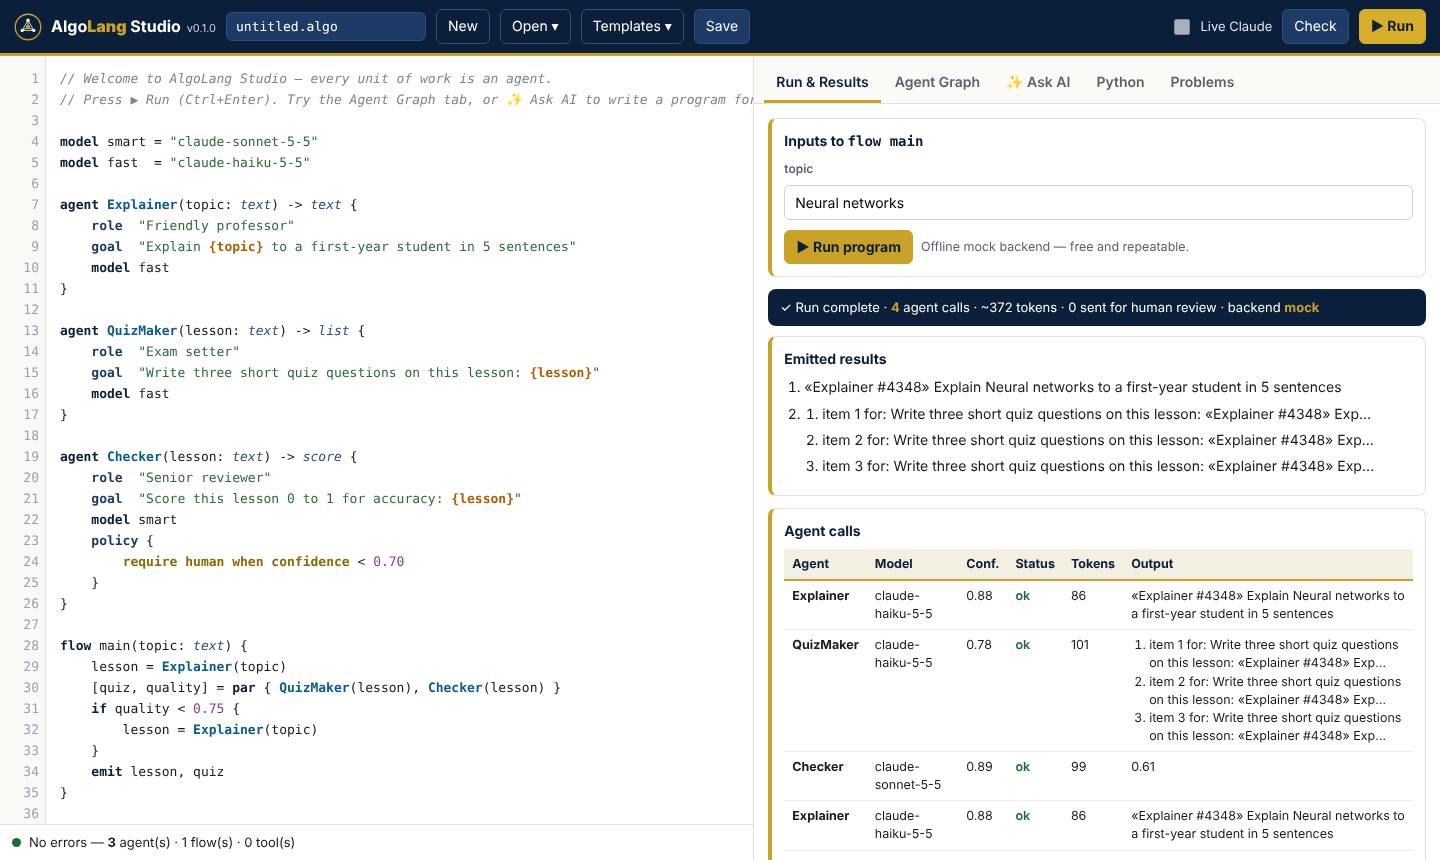
\includegraphics[width=\linewidth]{images/studio-run.png}
\caption{AlgoLang Studio after a run: the editor with highlighting and live error checking (left), and the inputs, emitted results and agent-call table (right).}
\label{fig:studio}
\end{figure}

\begin{center}
\small
\begin{tabularx}{\linewidth}{@{}L{3.2cm}Y@{}}
\toprule
\thead{Area} & \thead{What it does}\\
\goldrule
Editor & Syntax highlighting, line numbers, automatic indentation; errors marked in red in the margin as you type\\
\texttt{▶} Run (Ctrl+Enter) & Fills in a form for \code{flow main}'s inputs, runs, and shows results, confidences, human-review flags and the audit-log path\\
Agent Graph & Draws the flow top to bottom (Figure~\ref{fig:studiograph})\\
Ask AI & Describe a program in plain English; AI writes it (Section~\ref{sec:ask})\\
Templates & Start from any of six design patterns, no AI needed\\
Python & The code the compiler generates\\
Problems & Every compile error; click one to jump to its line\\
Open / Save & Your programs in the workspace folder, and the examples\\
Live Claude & Switches from the offline mock to real models (needs an API key)\\
\bottomrule
\end{tabularx}
\end{center}

\begin{figure}[ht]
\centering
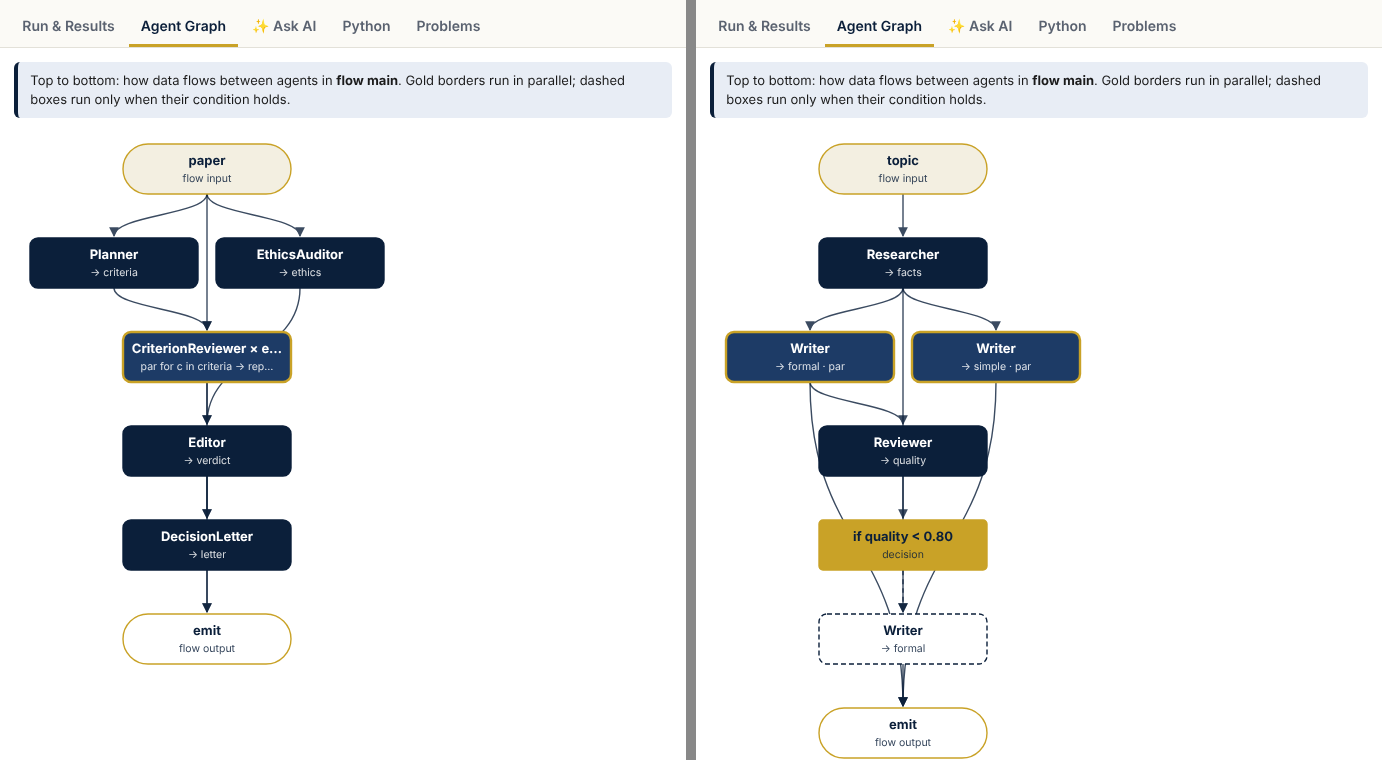
\includegraphics[width=0.92\linewidth]{images/studio-graphs.png}
\caption{Agent Graph for the paper-review program (left) and the research-brief program (right). Gold borders mark agents that run in parallel; the dashed box runs only when its condition holds.}
\label{fig:studiograph}
\end{figure}

\begin{note}
Studio listens only on \code{127.0.0.1} and refuses requests from other web sites, so other pages open in your browser cannot use it. Use \code{algo studio --port 9000} to choose a port, or \code{--no-browser} to start it without opening a window.
\end{note}

\section{Agentic: AI writes the program}
\label{sec:ask}

\code{algo ask} turns a description into a working \algolang\ program:

\begin{terminal}
$ algo ask "build a team that reviews a research paper and drafts a decision letter"
\end{terminal}

Behind the command is a small agentic loop, shown in Figure~\ref{fig:askloop}:

\begin{enumerate}
  \item A model receives your request together with a concise guide to \algolang's rules and an example.
  \item Its program is compiled by the real \algolang\ compiler.
  \item If there are errors, the exact compiler messages are sent back to the model to fix.
  \item This repeats up to three times. A program is accepted only when it compiles with \textbf{zero errors}; then it is saved and printed, and \code{--run} runs it immediately.
\end{enumerate}

\begin{figure}[ht]
\centering
\begin{tikzpicture}[
  st/.style={fill=navy,text=white,rounded corners=3pt,font=\sffamily\scriptsize,minimum width=24mm,minimum height=11mm,align=center},
  ok/.style={st,fill=strgreen},
  ch/.style={st,fill=gold,text=navy,font=\sffamily\scriptsize\bfseries},
  ar/.style={-{Stealth[length=2mm]},navy,line width=0.7pt}]
  \node[st] (r) {your\\request};
  \node[st,right=6mm of r] (m) {model writes\\AlgoLang};
  \node[ch,right=6mm of m] (c) {compiler\\checks};
  \node[ok,right=16mm of c] (s) {save + run\\(0 errors)};
  \draw[ar] (r) -- (m); \draw[ar] (m) -- (c); \draw[ar] (c) -- node[above,font=\sffamily\tiny]{no errors} (s);
  \draw[ar,cautionred] (c.south) -- ++(0,-6mm) -| node[pos=0.25,below,font=\sffamily\tiny,text=cautionred]{errors sent back (max 3 attempts)} (m.south);
\end{tikzpicture}
\caption{The write–compile–repair loop behind \code{algo ask} and Studio's Ask AI.}
\label{fig:askloop}
\end{figure}

The output shows each attempt. Here a first draft used an undefined placeholder and called a function; the compiler's messages were returned to the model, and the second attempt compiled:

\begin{terminal}
→ attempt 1: asking claude-sonnet-5-5 to write the program…
✗ attempt 1: 2 compile error(s) — sending them back to be fixed
    line 2: E109 agent Reviewer: goal mentions {manuscript} but there is no parameter 'manuscript'
    line 7: E101 'summarise' is not an agent — in AlgoLang every unit of work is an agent …
→ attempt 2: asking claude-sonnet-5-5 to write the program…
✓ attempt 2: compiles with no errors
\end{terminal}

\begin{ethics}[Generated programs still need review]
The compiler guarantees that a generated program is \emph{well-formed}: names, types, tools and policies are consistent. It cannot guarantee that the program does what you intended, or that its goals, thresholds and forbidden attributes are the right ones. Read every generated program before you run it live, exactly as you would review code written by a colleague.
\end{ethics}

\code{algo ask} needs \code{ANTHROPIC\_API\_KEY} and the \code{anthropic} package (Section~\ref{sec:live-setup}). The model can be changed with the environment variable \code{ALGO\_ASK\_MODEL}.

\section{Agentic without AI: the wizard}

\code{algo wizard} builds a program by asking six short questions. Pressing Enter accepts each default, so a complete program takes seconds:

\begin{terminal}
$ algo wizard
1. What should your AI system do [answer student questions about AI]: help students prepare for viva exams
2. Choose a design pattern:
   1. Pipeline — research, write, then edit, one after another
   2. Fan-out / fan-in — plan the parts, work on each in parallel, combine
   3. Committee — three experts answer in parallel, a judge decides
   4. Critic & revise — draft, score, redraft if the score is low
   5. Router — classify the input and send it to the right specialist
   6. Guardrail — safety check first, then do the work
   Pattern number [2]: 3
3. Name of the input (one word) [request]: question
4. Send low-confidence decisions to a human? (y/n) [y]:
   Confidence threshold (0-1) [0.75]: 0.8
5. Forbid protected attributes in decisions? (y/n) [y]:
   Which ones [gender, caste, religion, nationality]:
6. Token budget per agent [4000]: 3000
✓ wrote help_students_prepare_for_viva.algo (committee pattern) — it compiles with no errors.
\end{terminal}

The wizard's programs are built from the patterns of Chapter~\ref{ch:patterns}, with human review, budgets and protected-attribute rules placed on the agent that makes the final decision. They always compile, and they are a good starting point to edit by hand or in Studio.

\chapter{Your First Program}
\label{ch:first}

This chapter builds a small teaching assistant: one agent explains a topic, a second writes quiz questions on the explanation, and a third checks the explanation's accuracy. Along the way you will meet every part of an \algolang\ program.

\section{Create a starter}

\begin{terminal}
$ algo new mylesson
✓ created mylesson.algo
  next:  algo run mylesson.algo --arg "topic=Neural networks"
\end{terminal}

Open \file{mylesson.algo} in any editor:

\begin{algo}[title=mylesson.algo]
model smart = "claude-sonnet-5-5"
model fast  = "claude-haiku-5-5"

agent Explainer(topic: text) -> text {
    role  "Friendly professor"
    goal  "Explain {topic} to a first-year student in 5 sentences"
    model fast
}

agent QuizMaker(lesson: text) -> list {
    role  "Exam setter"
    goal  "Write three short quiz questions on this lesson: {lesson}"
    model fast
}

agent Checker(lesson: text) -> score {
    role  "Senior reviewer"
    goal  "Score this lesson 0 to 1 for accuracy: {lesson}"
    model smart
    policy {
        require human when confidence < 0.70
    }
}

flow main(topic: text) {
    lesson = Explainer(topic)
    [quiz, quality] = par { QuizMaker(lesson), Checker(lesson) }
    if quality < 0.75 {
        lesson = Explainer(topic)
    }
    emit lesson, quiz
}
\end{algo}

\section{Reading the program}

\begin{description}[style=nextline,leftmargin=1.2em,font=\sffamily\bfseries\color{navy}]
  \item[Models] \kw{model} gives a short name to a model identifier. Agents refer to the short name, so changing models later is a one-line edit.
  \item[Agents] Each \kw{agent} has typed parameters, a return type after \code{->}, and clauses. The \kw{goal} is the instruction the model receives; \code{\{topic\}} is replaced by the argument's value when the agent runs.
  \item[Return types] \code{Explainer} returns \kw{text}, \code{QuizMaker} a \kw{list}, and \code{Checker} a \kw{score}---a number from 0 to 1. Only scores and numbers can be compared.
  \item[Policy] \code{Checker} sends any result whose confidence is below 0.70 for human review.
  \item[Flow] \code{flow main} is the entry point. Its input \code{topic} comes from the command line.
  \item[Parallelism] \kw{par} runs \code{QuizMaker} and \code{Checker} at the same time; their results are bound to \code{quiz} and \code{quality} in order.
  \item[Branching] If the quality score is below 0.75, the explanation is regenerated.
  \item[Output] \kw{emit} returns the final values from the flow.
\end{description}

\section{Check, then run}

\begin{terminal}
$ algo check mylesson.algo
✓ mylesson.algo: 3 agents, 1 flow(s), 0 tool(s) — no errors

$ algo run mylesson.algo --arg "topic=Neural networks"
▶ flow main  run=a8a5732e  backend=mock
    topic = 'Neural networks'
  → Explainer          conf=0.88  «Explainer #4348» Explain Neural networks to a first-…
  → QuizMaker          conf=0.78  [3 items]
  → Checker            conf=0.89  0.61
  → Explainer          conf=0.88  «Explainer #4348» Explain Neural networks to a first-…
■ emitted:
    • «Explainer #4348» Explain Neural networks to a first-year student in 5 sentences
    • item 1 for: Write three short quiz questions on this lesson: …
    • item 2 for: Write three short quiz questions on this lesson: …
    • item 3 for: Write three short quiz questions on this lesson: …
■ 4 agent calls · ~372 tokens · 0 retries · 0 escalated · 0 blocked · audit → runs/mylesson.audit.jsonl
\end{terminal}

Each line beginning with \code{→} is one agent call, with its confidence and a preview of its output. The \code{Checker} scored the lesson 0.61, below the flow's 0.75 bar, so the \code{Explainer} ran a second time---four calls in total.

\begin{note}
On the mock backend an agent's output is a labelled echo of its goal, such as \code{«Explainer \#4348» Explain Neural networks…}. The number is a fingerprint of the input, so the same input always gives the same output and confidence. This makes runs repeatable for teaching and testing. Run with \code{--live} to get real model answers (Section~\ref{sec:live-setup}).
\end{note}

\section{What just happened}

Before running, \code{algo} compiled \file{mylesson.algo} to Python in \file{build/mylesson.py}, after checking every name, argument count, type, model and tool. At run time each agent call passed through the runtime's policy checks and was written to the audit log \file{runs/mylesson.audit.jsonl}---one JSON line per call, recording the model, a hash of the inputs, the confidence, the token count and the outcome. Chapter~\ref{ch:runtime} describes this in detail.

\section{Try it yourself}

\begin{enumerate}
  \item Change \code{Checker}'s threshold to \code{0.95} and run again. How many results are now escalated?
  \item Add a \code{Summariser(lesson: text) -> text} agent and \kw{emit} its output as a third value.
  \item Call an agent that does not exist, for example \code{x = Translate(lesson)}, and read the compiler's message.
\end{enumerate}


\docpart{The Language}
\chapter{Programs and Lexical Structure}
\label{ch:lexical}

\section{Source files}

An \algolang\ program is a single UTF-8 text file with the extension \file{.algo}. It consists of top-level declarations in any order:

\begin{center}
\small
\begin{tabularx}{\linewidth}{@{}L{2.6cm}L{4.2cm}Y@{}}
\toprule
\thead{Declaration} & \thead{Form} & \thead{Purpose}\\
\goldrule
\kw{model} & \code{model name = "id"} & Names a model identifier\\
\kw{tool} & \code{tool web.search} & Declares a capability agents may be granted\\
\kw{agent} & \code{agent N(p: t) -> t \{ … \}} & Declares a unit of work\\
\kw{flow} & \code{flow main(p: t) \{ … \}} & Orchestrates agents\\
\bottomrule
\end{tabularx}
\end{center}

Every program must contain exactly one \code{flow main}, which is where execution starts (error \errcode{E111} otherwise).

\section{Comments, whitespace and semicolons}

\begin{itemize}
  \item A comment starts with \code{//} and runs to the end of the line.
  \item Whitespace, including newlines, separates tokens and is otherwise ignored. Indentation has no meaning.
  \item Semicolons are allowed and ignored, so \code{a = A(x); b = B(a)} on one line is the same as two lines.
\end{itemize}

\section{Identifiers}

Identifiers match \code{[a-zA-Z\_][a-zA-Z0-9\_]*}. By convention agents use \code{PascalCase} (\code{Researcher}), and variables, parameters and models use \code{lower\_case} (\code{facts}, \code{smart}). Names of agents and flows share one namespace; defining the same name twice is error \errcode{E107}.

Tool names are \emph{dotted} identifiers with at least two parts, such as \code{web.search} or \code{file.read}.

\section{Keywords}

\begin{center}
\small
\begin{tabularx}{\linewidth}{@{}L{3.3cm}Y@{}}
\toprule
\thead{Group} & \thead{Keywords}\\
\goldrule
Declarations & \kw{model} \kw{tool} \kw{agent} \kw{flow}\\
Agent clauses & \kw{role} \kw{goal} \kw{uses} \kw{model} \kw{policy}\\
Policy rules & \kw{budget} \kw{tokens} \kw{retry} \kw{timeout} \kw{require} \kw{human} \kw{when} \kw{confidence} \kw{forbid}\\
Flow statements & \kw{par} \kw{for} \kw{in} \kw{if} \kw{else} \kw{emit}\\
Literals & \kw{true} \kw{false}\\
Types & \kw{text} \kw{score} \kw{list} \kw{json} \kw{bool}\\
\bottomrule
\end{tabularx}
\end{center}

\section{Literals}

\begin{itemize}
  \item \textbf{Strings} are enclosed in double quotes. Backslash escapes such as \code{\textbackslash n} and \code{\textbackslash"} are supported.
  \item \textbf{Numbers} are written as \code{6000} or \code{0.75}. Negative and exponent forms are not part of version 0.1.
  \item \textbf{Booleans} are \kw{true} and \kw{false}.
\end{itemize}

\section{Placeholders in goals}

Inside a \kw{goal} string, \code{\{name\}} is a placeholder for the parameter \code{name}. When the agent runs, the placeholder is replaced by the argument's value (a list is joined with \code{"; "}). The compiler checks that every placeholder names a real parameter (\errcode{E109}).

\begin{algo}
agent Translator(passage: text, language: text) -> text {
    goal "Translate into {language}, keeping technical terms: {passage}"
}
\end{algo}

\section{Operators}

\begin{center}
\small
\begin{tabularx}{\linewidth}{@{}L{3.3cm}Y@{}}
\toprule
\thead{Operator} & \thead{Use}\\
\goldrule
\code{->} & Separates an agent's parameters from its return type\\
\code{=} & Assignment in flows; default values in parameters; keyword arguments\\
\code{<} \code{<=} \code{>} \code{>=} \code{==} \code{!=} & Comparisons in \kw{if} conditions\\
\code{[ , ]} & Binds several results of a \kw{par} block\\
\bottomrule
\end{tabularx}
\end{center}

\algolang\ has no arithmetic or string operators. Computation is done by agents; flows only route values between them.

\chapter{Types and Results}
\label{ch:types}

\section{The five types}

Every agent parameter, agent return value and flow input has one of five types.

\begin{center}
\small
\begin{tabularx}{\linewidth}{@{}L{1.6cm}L{4.4cm}YL{2.4cm}@{}}
\toprule
\thead{Type} & \thead{Meaning} & \thead{Typical use} & \thead{Mock value}\\
\goldrule
\kw{text} & Free text & Facts, drafts, summaries, letters & labelled echo of the goal\\
\kw{score} & Number from 0 to 1 & Quality, risk, acceptance likelihood & 0.55--0.95\\
\kw{list} & Ordered list of items & Criteria, sub-tasks, questions & 3--4 items\\
\kw{json} & Structured object & Extracted fields, records & small object\\
\kw{bool} & True or false & Pass/fail checks & true or false\\
\bottomrule
\end{tabularx}
\end{center}

An unknown type name is error \errcode{E105}. Literals have their own types: a string literal is \kw{text}, \kw{true} and \kw{false} are \kw{bool}, and a number literal is a \emph{number}, which can be compared with scores.

\section{Where types matter}

The compiler uses types in three places:

\begin{enumerate}
  \item \textbf{Comparisons.} An \kw{if} condition may compare only scores, numbers and booleans. Comparing text is error \errcode{E110}:
\begin{algo}
summary = Summariser(doc)          // text
if summary < 0.5 { emit summary }  // E110: 'summary' is text, not a score
\end{algo}
  \item \textbf{Parallel loops.} \kw{par for} iterates over a \kw{list}; anything else is error \errcode{E114}.
  \item \textbf{Variables.} Each variable takes the type of the agent that produced it. A \kw{par} block bound to a single name produces a \kw{list}; the loop variable of \kw{par for} is \kw{text}.
\end{enumerate}

\begin{caution}
In version 0.1 the compiler does not yet check that an argument's type matches the parameter's declared type (for example, passing a \kw{list} where \kw{text} is expected). Lists passed to text parameters are joined with \code{"; "} when the goal is rendered. Full argument type checking is planned for version 0.2.
\end{caution}

\section{Results: value plus provenance}

Every agent call returns a \emph{Result}, not a bare value. A Result carries:

\begin{center}
\small
\begin{tabularx}{\linewidth}{@{}L{2.6cm}Y@{}}
\toprule
\thead{Field} & \thead{Meaning}\\
\goldrule
\code{value} & The agent's output, of its declared return type\\
\code{confidence} & A number from 0 to 1 reported with the output\\
\code{agent} & Which agent produced it\\
\code{call\_id} & A short identifier linking it to its audit record\\
\code{status} & \code{ok}, \code{escalated} (sent for human review) or \code{approved} (a human approved it)\\
\bottomrule
\end{tabularx}
\end{center}

In flows you use a Result exactly like its value: passing it to another agent passes the value, and comparing it compares the value. The extra fields are visible in the audit log, in notebooks (\code{algo\_calls}), and to Python code that uses the generated program.

\begin{ethics}[Uncertainty is part of the answer]
Hiding uncertainty encourages over-trust in AI output. By making confidence part of every result, \algolang\ makes it natural to route uncertain results to people (Chapter~\ref{ch:policies}) and to report uncertainty to end users. Remember, however, that a model's \emph{self-reported} confidence is not a calibrated probability (Section~\ref{sec:limits}).
\end{ethics}

\section{Flow inputs}

Flow parameters are declared with types like agent parameters:

\begin{algo}
flow main(topic: text, audience: text) { ... }
\end{algo}

Values are supplied on the command line with \code{--arg "name=value"}, in notebooks with the same option, or interactively when omitted.

\begin{note}
In version 0.1 every flow input arrives as text, whatever its declared type. Declare flow inputs as \kw{text} and let an agent convert them if needed.
\end{note}

\chapter{Models, Tools and Agents}
\label{ch:declarations}

\section{Models}

\begin{algo}
model smart = "claude-sonnet-5-5"
model fast  = "claude-haiku-5-5"
\end{algo}

A \kw{model} declaration binds a short name to a model identifier. Agents select a model by short name with the \kw{model} clause; an unknown name is error \errcode{E106}. An agent without a \kw{model} clause uses \code{claude-sonnet-5-5}.

\begin{tip}
Name models by their role in your system---\code{smart}, \code{fast}, \code{cheap}---not by product. When a new model is released you change one line, and every agent that uses that role moves with it.
\end{tip}

\section{Tools}

\begin{algo}
tool web.search
tool file.read
\end{algo}

A \kw{tool} declaration announces a capability that the program may grant. Declaring a tool gives it to no one: each agent must list the tools it needs in a \kw{uses} clause, and listing a tool that was never declared is error \errcode{E104}.

\begin{ethics}[Least privilege]
An agent can only be granted capabilities that the program declares openly at the top of the file, and only the agents that list a tool receive it. A reviewer can see every capability of a program, and which agent holds it, without reading any agent's code. This is the security principle of least privilege applied to AI agents.
\end{ethics}

\begin{caution}
Tools are \emph{capability declarations} that the compiler enforces. Since version 0.2 they are also executable: the runtime calls the registered Python function (built-ins \code{calc.eval}, \code{file.read}, \code{kb.search}, or your own plugin) and records every call in the audit log (Chapter~\ref{ch:enterprise}). MCP bindings are planned for version 0.3.
\end{caution}

\section{Agents}

An agent declaration has a name, typed parameters, a return type and a body of clauses:

\begin{algo}[title=agent anatomy]
agent CriterionReviewer(criterion: text, paper: text, depth: text = "detailed") -> text {
    role   "Domain reviewer"
    goal   "Give a {depth} review of {paper} strictly on: {criterion}"
    uses   file.read, web.search
    model  fast
    policy {
        budget tokens 4000
        retry 1
    }
}
\end{algo}

\subsection{Parameters}

Each parameter is \code{name: type}, optionally with a default literal: \code{tone: text = "academic"}. A parameter with a default may be omitted by the caller. Parameter names must not appear in the agent's \kw{forbid} list (\errcode{E108}).

\subsection{Clauses}

\begin{center}
\small
\begin{tabularx}{\linewidth}{@{}L{1.6cm}L{1.8cm}Y@{}}
\toprule
\thead{Clause} & \thead{Required} & \thead{Meaning}\\
\goldrule
\kw{goal} & \textbf{yes} & The work the agent must do, in plain language. Placeholders \code{\{param\}} are filled when it runs. Missing goal: \errcode{E112}.\\
\kw{role} & no & The capacity in which the agent acts; becomes its persona (system prompt in live mode).\\
\kw{uses} & no & Comma-separated tools the agent may use; each must be declared (\errcode{E104}).\\
\kw{model} & no & Short name of a declared model (\errcode{E106}).\\
\kw{policy} & no & Governance rules---see Chapter~\ref{ch:policies}.\\
\bottomrule
\end{tabularx}
\end{center}

Clauses may appear in any order. A clause may be repeated; for \kw{uses} the lists are combined, and for the others the last one wins.

\subsection{What the model receives}

At run time the runtime renders the agent into a prompt with three parts:

\begin{plaincode}[title=rendered prompt]
ROLE: Domain reviewer
GOAL: Give a detailed review of LG-CEF … strictly on: Methodology & rigour
TOOLS: file.read, web.search
\end{plaincode}

In live mode the role becomes the system persona and the model is asked to reply with a JSON object holding its \code{value} and \code{confidence}, in the shape required by the agent's return type.

\section{Writing good agents}

\begin{enumerate}
  \item \textbf{One job per agent.} If a goal contains ``and then'', split it into two agents and connect them in a flow.
  \item \textbf{Write goals as instructions to a capable colleague.} State the output you expect: length, format, audience.
  \item \textbf{Choose the narrowest return type.} If the flow will branch on it, return a \kw{score} or \kw{bool}, not \kw{text}.
  \item \textbf{Grant the fewest tools.} An agent that only rewrites text needs no tools at all.
  \item \textbf{Always set a budget} for agents that will run live.
  \item \textbf{Gate decisions that affect people} with \kw{require human when confidence < …}.
\end{enumerate}

\chapter{Policies}
\label{ch:policies}

A \kw{policy} block attaches governance rules to an agent. Policies are part of the agent's declaration, so they travel with it, appear in its audit records and cannot be forgotten by a caller.

\begin{algo}
agent Editor(reports: list, ethics: text) -> score {
    role  "Editor-in-Chief"
    goal  "Weigh {reports} and {ethics}; score acceptance likelihood 0 to 1"
    policy {
        budget tokens 6000
        retry 2
        timeout 60
        require human when confidence < 0.75
        forbid gender, caste, religion, nationality
    }
}
\end{algo}

\section{Summary of rules}

\begin{center}
\small
\begin{tabularx}{\linewidth}{@{}L{4.6cm}L{2.2cm}Y@{}}
\toprule
\thead{Rule} & \thead{Checked} & \thead{Effect}\\
\goldrule
\kw{budget tokens} \code{N} & run time & Stops the call before it is sent if the prompt is estimated above \code{N} tokens; in live mode also caps the reply length\\
\kw{retry} \code{N} & run time & Retries a failed call up to \code{N} more times\\
\kw{timeout} \code{S} & run time & Treats a call that took longer than \code{S} seconds as failed\\
\kw{require human when confidence <} \code{X} & run time & Marks a result with confidence below \code{X} as \code{escalated}, or asks a person to approve it\\
\kw{forbid} \code{a, b, …} & compile \emph{and} run time & Rejects agents that take a forbidden attribute as a parameter; stops calls whose inputs mention one\\
\bottomrule
\end{tabularx}
\end{center}

\section{Token budgets}

\code{budget tokens N} protects against runaway cost. Before every call the runtime estimates the prompt's size (about four characters per token). If the estimate exceeds \code{N}, the call is not sent: the run stops with a policy violation. In live mode the budget also sets the maximum length of the model's reply (capped at 8,000 tokens; without a budget the reply is limited to 2,000 tokens).

\begin{tip}
A budget that is too small for an agent's normal input is a design signal: the agent is being asked to do too much at once. Split the work, or summarise the input with another agent first.
\end{tip}

\section{Retries and timeouts}

\code{retry N} makes the runtime try a failed call up to \code{N} more times---useful for transient network or service errors. Policy violations are never retried. \code{timeout S} marks a call as failed if it took longer than \code{S} seconds; the check is made when the call returns, and a timed-out call can then be retried.

\section{Human oversight}

\code{require human when confidence < X} is the human-in-the-loop gate. When an agent's result has confidence below \code{X}:

\begin{itemize}
  \item By default the result is marked \code{escalated}: the flow continues, the run summary counts the escalation, and the audit record carries \code{"status": "escalated"} so that a person can review it afterwards.
  \item With \code{--interactive} (terminal or notebook) the run pauses and shows the result. Typing \code{y} records \code{approved}; any other answer keeps it \code{escalated}.
\end{itemize}

\begin{terminal}
  → Reviewer           conf=0.68  0.78  ⚠ ESCALATED to human (conf < 0.70)
\end{terminal}

\begin{ethics}[Meaningful human oversight]
Oversight is only meaningful if people see the right cases. Put the gate on the agents whose outputs affect people---decisions, scores, letters---and choose thresholds deliberately. Review the escalation count in every run summary: if it is always zero, the threshold may be too low to matter; if it is always high, the agent or its model may not be fit for the task.
\end{ethics}

\section{Forbidden attributes}
\label{sec:forbid}

\code{forbid} names attributes that must not influence an agent's work---typically protected characteristics such as gender, caste, religion, nationality or age. It acts twice:

\begin{enumerate}
  \item \textbf{At compile time}, an agent may not declare a parameter with a forbidden name (\errcode{E108}):
\begin{terminal}
  line 12: E108 agent Screener takes forbidden attribute 'caste' as an input
\end{terminal}
  \item \textbf{At run time}, before each call, the runtime searches the rendered prompt (role, goal with all arguments filled in, and tools) for each forbidden word, as a whole word and ignoring case. If one is found, the call is not made and the run stops:
\begin{terminal}
  → EthicsAuditor      conf=0.79  «EthicsAuditor #1139» Check Does author nationality …
✗ POLICY VIOLATION: Editor: input mentions forbidden attribute 'nationality'
\end{terminal}
\end{enumerate}

The blocked call is recorded in the audit log with \code{"status": "blocked"} and the reason, and the program exits with code~2.

\begin{caution}
The run-time check is \emph{lexical}: it finds the forbidden words themselves, not their proxies. A surname, a home town or a school can still reveal caste, religion or nationality. \kw{forbid} is a strong safeguard against accidental and obvious leakage and a clear statement of intent, but it is not a guarantee of fairness. Combine it with careful input design and with audits of outcomes across groups (Chapter~\ref{ch:responsible}).
\end{caution}

\section{Where policies are recorded}

Every audit record includes the agent's full policy, so a reviewer can see which rules were in force for each call:

\begin{plaincode}[title=from an audit record]
"status": "ok",
"policy": {"budget_tokens": 6000, "retry": 2}
\end{plaincode}

\chapter{Flows}
\label{ch:flows}

A \kw{flow} connects agents. It has typed parameters and a body of statements, and it can do exactly five things: call an agent, run agents in parallel, map an agent over a list in parallel, branch on a comparison, and emit results. It cannot compute anything itself, and it cannot be called---every program's entry point is \code{flow main}.

\section{Calling agents}

\begin{algo}
facts  = Researcher(topic)                       // positional
brief  = Writer(facts, tone = "plain-English")   // positional + keyword
letter = DecisionLetter(verdict = v, reports = r) // keywords in any order
\end{algo}

Positional arguments bind to parameters in order; keyword arguments bind by name. Parameters with defaults may be omitted. The compiler reports too many arguments, unknown names, duplicates and missing required arguments as \errcode{E102}.

A call may also stand alone as a statement when only its effect matters, for example an agent that files a report:

\begin{algo}
Notifier(summary)
\end{algo}

\section{Variables}

Assignment binds a name to an agent's result. Variables need no declaration; a variable's type is its agent's return type. Using a name that has not been assigned (and is not a flow input) is \errcode{E103}. A variable may be reassigned, as in the redraft pattern:

\begin{algo}
draft = Writer(facts)
if Reviewer(draft) < 0.8 { draft = Writer(facts, tone = "rigorous") }
\end{algo}

\section{Parallel blocks: \kw{par}}

\begin{algo}[]
[formal, simple, hindi] = par {
    Writer(facts),
    Writer(facts, tone = "plain-English"),
    Translator(facts, language = "Hindi")
}
\end{algo}

All calls inside \kw{par} run at the same time. The bracketed names receive the results in the order the calls are written, whatever order they finish in. The number of names must equal the number of calls (\errcode{E113}). Assigned to a single name, a \kw{par} block yields a \kw{list}:

\begin{algo}
opinions = par { ExpertA(q), ExpertB(q), ExpertC(q) }   // list of three results
\end{algo}

\section{Parallel map: \kw{par for}}

\begin{algo}
criteria = Planner(paper)                                    // list
reports  = par for c in criteria { CriterionReviewer(c, paper) }
\end{algo}

\kw{par for} runs one call per item of a list, all concurrently, and collects the results in the list's order. The source must be a \kw{list} (\errcode{E114}); the loop variable is visible only inside the braces. This is the ``fan-out / fan-in'' pattern of multi-agent systems in one line.

\section{Branching: \kw{if} and \kw{else}}

\begin{algo}
verdict = Editor(reports, ethics)
if verdict >= 0.5 {
    letter = AcceptLetter(reports)
} else {
    letter = RejectLetter(reports)
}
\end{algo}

A condition compares two values with \code{<}, \code{<=}, \code{>}, \code{>=}, \code{==} or \code{!=}. Each side may be a variable, a number or an agent call that returns a \kw{score}, so \code{if Reviewer(draft) < 0.8 \{ … \}} is valid. Only scores, numbers and booleans can be compared (\errcode{E110}).

\section{Returning results: \kw{emit}}

\begin{algo}
emit verdict, letter
\end{algo}

\kw{emit} adds values to the flow's output. A flow may emit several times; the outputs accumulate in order. The terminal shows them after the run; notebooks place them in \code{algo\_result}; Python callers receive them as a list.

\section{Complete example}

\begin{algo}[title=paper\_review.algo — flow]
flow main(paper: text) {
    criteria = Planner(paper)
    reports  = par for c in criteria { CriterionReviewer(c, paper) }
    ethics   = EthicsAuditor(paper)
    verdict  = Editor(reports, ethics)
    letter   = DecisionLetter(reports, verdict)
    emit verdict, letter
}
\end{algo}

The notebook extension draws this flow as a graph (Chapter~\ref{ch:notebooks}). Its shape is shown in Figure~\ref{fig:paperflow}.

\begin{figure}[ht]
\centering
\begin{tikzpicture}[
  node distance=7mm and 9mm,
  ag/.style={draw=none,fill=navy,text=white,rounded corners=3pt,font=\sffamily\footnotesize,
             minimum height=9mm,align=center,inner xsep=6pt},
  pa/.style={ag,fill=navy2,draw=gold,line width=1.2pt},
  io/.style={ellipse,fill=goldlight,draw=gold,font=\sffamily\footnotesize,text=navy,minimum height=8mm},
  ar/.style={-{Stealth[length=2.2mm]},navy,line width=0.7pt}]
  \node[io] (in) {paper};
  \node[ag,right=of in,yshift=9mm] (plan) {Planner\\[-1pt]{\scriptsize → criteria}};
  \node[pa,right=of plan] (rev) {CriterionReviewer × each\\[-1pt]{\scriptsize par for c in criteria}};
  \node[ag,below=10mm of rev] (eth) {EthicsAuditor\\[-1pt]{\scriptsize → ethics}};
  \node[ag,right=of rev,yshift=-9mm] (ed) {Editor\\[-1pt]{\scriptsize → verdict}};
  \node[ag,above=8mm of ed] (dl) {DecisionLetter\\[-1pt]{\scriptsize → letter}};
  \node[io,right=of ed,xshift=4mm,yshift=5mm] (out) {emit};
  \draw[ar] (in) -- (plan); \draw[ar] (plan) -- (rev); \draw[ar] (in) |- (eth);
  \draw[ar] (in.east) -- ++(4mm,0) |- (rev.west);
  \draw[ar] (rev) -- (ed); \draw[ar] (eth) -- (ed); \draw[ar] (rev) -- (dl); \draw[ar] (ed) -- (dl);
  \draw[ar] (ed) -- (out); \draw[ar] (dl) -- (out);
\end{tikzpicture}
\caption{Data flow of \file{paper\_review.algo}. The gold-edged node runs once per criterion, in parallel.}
\label{fig:paperflow}
\end{figure}

\chapter{Compile-Time Errors}
\label{ch:errors}

The compiler checks the whole program before generating any code and reports \emph{every} error it finds, each with a code and a line number. A program with errors is never built or run.

\begin{terminal}
$ algo check examples/bad_example.algo
✗ bad_example.algo: 8 error(s)
  line 5: E109 agent Summariser: goal mentions {document} but there is no parameter 'document'
  line 5: E104 agent Summariser uses tool 'email.send', which is not declared (add `tool email.send`)
  line 5: E106 agent Summariser: unknown model 'turbo'
  line 12: E108 agent Screener takes forbidden attribute 'caste' as an input
  line 19: E102 Summariser takes 1 argument(s) (doc), got 2 positional
  line 20: E101 'summarise_text' is not an agent — in AlgoLang every unit of work is an agent …
  line 21: E110 's' is text, not a score — only scores/numbers can be compared
  line 22: E103 undefined variable 'missing'
\end{terminal}

Errors about an agent's declaration are reported at the line where the agent starts.

\newcommand{\errhead}[2]{\subsection*{\errcode{#1}\enspace\textcolor{navy}{#2}}}

\section{Error catalogue}

\errhead{E100}{Syntax error}
The source does not match the grammar. The message shows the line and column with a pointer. Common causes: a missing \code{\}}, a missing \code{->} return type, an unquoted goal, or a keyword used as a name.

\errhead{E101}{Not an agent}
A call names something that is not a declared agent. This is \algolang's central rule. If the name is a flow, the message says that flows orchestrate and cannot be called.
\begin{algo}
t = summarise_text(doc)   // E101 — declare an agent instead
\end{algo}
\textbf{Fix:} declare \code{agent summarise\_text(doc: text) -> text \{ goal "…" \}}, or call an existing agent.

\errhead{E102}{Wrong arguments}
Too many positional arguments, an unknown keyword, a parameter given twice, or a required parameter missing.
\begin{algo}
s = Summariser(doc, doc)        // takes 1 argument(s) (doc), got 2 positional
w = Writer(facts, style = "x")  // Writer has no parameter 'style'
\end{algo}

\errhead{E103}{Undefined variable}
A name is used before it is assigned and is not a flow input. Check spelling and statement order.

\errhead{E104}{Undeclared tool}
An agent \kw{uses} a tool that the program never declares. \textbf{Fix:} add \code{tool email.send} at top level---a visible, reviewable decision to grant that capability.

\errhead{E105}{Unknown type}
A parameter or return type is not one of \kw{text}, \kw{score}, \kw{list}, \kw{json}, \kw{bool}.

\errhead{E106}{Unknown model}
An agent's \kw{model} clause names a model that was not declared with \kw{model}.

\errhead{E107}{Defined twice}
Two agents or flows share a name. Agents and flows share one namespace.

\errhead{E108}{Forbidden attribute as input}
An agent declares a parameter whose name appears in its own \kw{forbid} list.
\begin{algo}
agent Screener(caste: text) -> score {   // E108
    goal "Score applicant {caste}"
    policy { forbid caste }
}
\end{algo}
\textbf{Fix:} remove the parameter. If the attribute is genuinely needed---for example, to \emph{audit} outcomes across groups---give that job to a separate auditing agent whose policy does not forbid it, and document why.

\errhead{E109}{Unknown placeholder}
A \kw{goal} contains \code{\{name\}} but the agent has no parameter called \code{name}. Usually a typo, as in \code{\{document\}} for parameter \code{doc}.

\errhead{E110}{Comparing a non-score}
An \kw{if} condition compares a value that is not a score, number or boolean---typically \kw{text}. \textbf{Fix:} add an agent that returns a \kw{score} and compare that.

\errhead{E111}{No entry point}
The program has no \code{flow main}.

\errhead{E112}{Agent without a goal}
Every agent must state its work in a \kw{goal} clause.

\errhead{E113}{Mismatched parallel binding}
\code{[a, b] = …} needs a \kw{par} block on the right with the same number of calls.

\errhead{E114}{\kw{par for} over a non-list}
The source of \kw{par for} must be a \kw{list}, such as the output of a planning agent.

\errhead{E115}{Tool not allowed by organisation policy}
An agent \kw{uses} a tool that is missing from \code{allowed\_tools} in \file{algo.config.json} (Chapter~\ref{ch:enterprise}). Ask your administrator to approve the tool, or remove it. Org-forbidden attributes are reported as \errcode{E108}, before anything runs.

\section{Run-time outcomes}

Some problems can only be detected while the program runs. They are not compile errors; each stops the run with a clear message and an exit code (Chapter~\ref{ch:cli}).

\begin{center}
\small
\begin{tabularx}{\linewidth}{@{}L{4.3cm}L{1.3cm}Y@{}}
\toprule
\thead{Outcome} & \thead{Exit} & \thead{Cause}\\
\goldrule
Policy violation & 2 & A forbidden attribute in an agent's input, or a prompt over its token budget\\
Agent call failed & 3 & The model or service failed after all retries, or a timeout\\
Missing input / bad option & 1 & A flow input was not supplied, or \code{--arg} was not \code{name=value}\\
\bottomrule
\end{tabularx}
\end{center}


\docpart{Toolchain and Runtime}
\chapter{The \texttt{algo} Command}
\label{ch:cli}

All work with \algolang\ outside notebooks goes through one command, \code{algo}. On Windows it is \file{algo.bat}; on Linux and macOS it is the shell script \file{algo}. Both use the private \file{.venv} created by the installer when it exists.

\begin{terminal}
$ algo --help
usage: algo [-h] [--version] command ...

AlgoLang 0.2.0 — every unit of work is an agent

positional arguments:
  command
    check     check a program for errors
    build     compile to Python
    run       compile and run flow main
    new       create a starter program
    doctor    check that the environment is ready
    notebook  open the AlgoLang notebook in Jupyter (installs Jupyter if needed)
\end{terminal}

\section{Commands}

\begin{center}
\small
\begin{tabularx}{\linewidth}{@{}L{5.2cm}Y@{}}
\toprule
\thead{Command} & \thead{What it does}\\
\goldrule
\code{algo check FILE.algo} & Parses and checks the program; reports all errors; writes nothing\\
\code{algo build FILE.algo [-o OUT.py]} & Compiles to Python; default output \file{build/FILE.py} next to the source\\
\code{algo run FILE.algo [options]} & Compiles, then runs \code{flow main}\\
\code{algo new NAME} & Creates \file{NAME.algo} from a ready-to-run three-agent template\\
\code{algo doctor} & Checks Python, the parser, live-mode readiness and a compiler self-test\\
\code{algo notebook} & Opens \file{AlgoLang\_Notebook.ipynb} in Jupyter, installing Jupyter the first time\\
\code{algo} & Numbered menu of every option\\
\code{algo shell} & Interactive shell: type declarations one at a time\\
\code{algo studio [--port N]} & AlgoLang Studio, the graphical IDE in your browser\\
\code{algo ask "…" [-o F] [--run]} & AI writes a program from a description (compile-and-repair loop)\\
\code{algo wizard} & Build a program by answering questions, no AI needed\\
\code{algo --version} & Prints the version\\
\bottomrule
\end{tabularx}
\end{center}

\section{Options for \texttt{run}}

\begin{center}
\small
\begin{tabularx}{\linewidth}{@{}L{4.4cm}Y@{}}
\toprule
\thead{Option} & \thead{Meaning}\\
\goldrule
\code{--arg "name=value"} & Supplies a flow input; repeat for several inputs. Inputs not supplied are asked for interactively\\
\code{--live} & Runs agents on real Claude models (needs \code{ANTHROPIC\_API\_KEY})\\
\code{--interactive} & Pauses on low-confidence results for human approval\\
\code{--audit-dir DIR} & Writes audit logs to \code{DIR} (default \file{runs})\\
\bottomrule
\end{tabularx}
\end{center}

\begin{terminal}
$ algo run examples/paper_review.algo \
      --arg "paper=LG-CEF: lesion-guided ensemble for DR grading" \
      --interactive --audit-dir audit/2026-10
\end{terminal}

\section{Exit codes}

\begin{center}
\small
\begin{tabularx}{\linewidth}{@{}L{1.3cm}Y@{}}
\toprule
\thead{Code} & \thead{Meaning}\\
\goldrule
0 & Success\\
1 & Compile errors, a missing file or input, or a malformed option\\
2 & A policy violation stopped the run\\
3 & An agent call failed after its retries\\
\bottomrule
\end{tabularx}
\end{center}

Scripts and continuous-integration jobs can rely on these codes; for example, a CI job can run \code{algo check} on every \file{.algo} file and fail the build on exit code 1.

\section{Environment variables}

\begin{center}
\small
\begin{tabularx}{\linewidth}{@{}L{4.3cm}Y@{}}
\toprule
\thead{Variable} & \thead{Meaning}\\
\goldrule
\code{ANTHROPIC\_API\_KEY} & API key for live mode\\
\code{ALGO\_HOME} & Folder containing the runtime; set automatically by \code{algo}\\
\code{ALGO\_LIVE=1} & Live mode (set by \code{--live})\\
\code{ALGO\_INTERACTIVE=1} & Interactive human review (set by \code{--interactive})\\
\code{ALGO\_AUDIT\_DIR} & Audit-log folder (set by \code{--audit-dir})\\
\bottomrule
\end{tabularx}
\end{center}

\section{Running compiled programs directly}

\code{algo build} produces an ordinary Python script that can be run, scheduled or shipped without the compiler:

\begin{terminal}
$ algo build research_brief.algo
✓ compiled research_brief.algo → build/research_brief.py
$ python build/research_brief.py --topic "Federated learning in IoT"
\end{terminal}

The script needs only \file{algoruntime.py}, found through \code{ALGO\_HOME} or the path recorded at compile time.

\chapter{Runtime Semantics}
\label{ch:runtime}

This chapter defines precisely what happens when a compiled program runs. The reference implementation is \file{algoruntime.py}.

\section{Lifecycle of a run}

\begin{enumerate}
  \item The runtime is created with the program's name and a fresh \emph{run identifier}; models and tools are registered; the backend is chosen (mock, or live when \code{ALGO\_LIVE=1}).
  \item Each agent declaration becomes a governed callable.
  \item \code{flow main} starts with its inputs and prints a header line.
  \item Statements execute in order; \kw{par} and \kw{par for} execute their calls concurrently.
  \item Emitted values accumulate; at the end the runtime prints them with a summary line: calls, estimated tokens, retries, escalations and blocked calls.
\end{enumerate}

\section{Lifecycle of an agent call}
\label{sec:callsteps}

Every agent call passes through the same seven steps, shown in Figure~\ref{fig:callsteps}.

\begin{figure}[ht]
\centering
\begin{tikzpicture}[
  st/.style={fill=navy,text=white,rounded corners=3pt,font=\sffamily\scriptsize,
             minimum width=19mm,minimum height=11mm,align=center,inner sep=3pt},
  ch/.style={st,fill=gold,text=navy,font=\sffamily\scriptsize\bfseries},
  ar/.style={-{Stealth[length=2mm]},navy,line width=0.7pt},
  stop/.style={font=\sffamily\scriptsize,text=cautionred,align=center}]
  \node[st] (s1) {1. bind\\arguments};
  \node[st,right=4mm of s1] (s2) {2. render\\prompt};
  \node[ch,right=4mm of s2] (s3) {3. forbid\\check};
  \node[ch,right=4mm of s3] (s4) {4. budget\\check};
  \node[st,right=4mm of s4] (s5) {5. call model\\(retry, timeout)};
  \node[ch,below=9mm of s5] (s6) {6. human\\gate};
  \node[st,left=4mm of s6] (s7) {7. audit +\\return Result};
  \foreach \a/\b in {s1/s2,s2/s3,s3/s4,s4/s5,s5/s6,s6/s7} \draw[ar] (\a) -- (\b);
  \node[stop,below=3mm of $(s3.south)!0.5!(s4.south)$] {policy violation: blocked → exit 2};
  \node[stop,above=2.5mm of s5] {fails after retries → exit 3};
\end{tikzpicture}
\caption{The seven steps of every agent call. Gold steps enforce policy.}
\label{fig:callsteps}
\end{figure}

\begin{enumerate}
  \item \textbf{Bind arguments.} Positional and keyword arguments are matched to parameters; defaults fill the rest. Results passed as arguments contribute their values.
  \item \textbf{Render the prompt.} Placeholders in the goal are replaced with argument values (lists joined with \code{"; "}), and the prompt is assembled from role, goal and tools.
  \item \textbf{Forbid check.} If the prompt contains a forbidden attribute as a whole word (ignoring case), the call is recorded as \code{blocked} and a policy violation stops the run.
  \item \textbf{Budget check.} If the prompt's estimated size (characters ÷ 4) exceeds the token budget, the call is recorded as \code{blocked} and a policy violation stops the run.
  \item \textbf{Call the model} through the backend, retrying failures up to the \kw{retry} count and treating calls longer than \kw{timeout} as failures. If all attempts fail, the call is recorded as \code{failed} and the run stops.
  \item \textbf{Human gate.} If the confidence is below the \kw{require human} threshold, the Result's status becomes \code{escalated}, or \code{approved} if a reviewer approves it in interactive mode.
  \item \textbf{Audit and return.} One audit record is written and the Result is returned to the flow.
\end{enumerate}

\section{Concurrency}

\kw{par} and \kw{par for} submit their calls to a thread pool sized to the number of calls and wait for all of them. Results are returned in source order, not completion order, so programs are deterministic in structure even when timing varies. Console output and audit writes are serialised by a lock, so lines never interleave.

\begin{note}
If one call in a parallel group fails or violates a policy, the error stops the run after the group's other calls have finished; their audit records are still written.
\end{note}

\section{Backends}

\begin{center}
\small
\begin{tabularx}{\linewidth}{@{}L{2.2cm}YY@{}}
\toprule
\thead{} & \thead{Mock (default)} & \thead{Live (\code{--live})}\\
\goldrule
Purpose & Teaching, testing, CI, offline demos & Real work\\
Cost & Free & API credits\\
Determinism & Same input → same output & Varies between runs\\
Output & Labelled echo of the goal; shaped by return type & The model's answer, in a JSON envelope\\
Confidence & Derived from a hash of the input (0.62--0.95) & Reported by the model\\
Tokens & Estimated & Counted by the API\\
\bottomrule
\end{tabularx}
\end{center}

In live mode, the role becomes the system persona, and the model is instructed to reply only with JSON of the form \code{\{"value": …, "confidence": …\}}, where the value's shape matches the return type (a number for \kw{score}, an array for \kw{list}, and so on). If the reply contains no JSON object, the whole reply is used as the value with confidence 0.5.

\section{The audit log}
\label{sec:audit}

Every agent call appends one JSON line to \file{<audit-dir>/<program>.audit.jsonl}:

\begin{plaincode}[title=one audit record (pretty-printed)]
{
  "call": "d5a1ba",
  "agent": "Researcher",
  "model": "claude-sonnet-5-5",
  "backend": "mock",
  "inputs_sha": "23cd4baf6ab210a5",
  "returns": "text",
  "confidence": 0.83,
  "tokens": 93,
  "status": "ok",
  "tools": ["web.search"],
  "policy": {"budget_tokens": 6000, "retry": 2},
  "run": "832d55bb",
  "program": "research_brief",
  "ts": "2026-10-28T11:20:13"
}
\end{plaincode}

\begin{center}
\small
\begin{tabularx}{\linewidth}{@{}L{2.4cm}Y@{}}
\toprule
\thead{Field} & \thead{Meaning}\\
\goldrule
\code{run}, \code{call} & Identifiers of the run and of this call\\
\code{program}, \code{agent} & What ran\\
\code{model}, \code{backend} & Which model, and mock or live\\
\code{inputs\_sha} & First 16 hex digits of the SHA-256 hash of the full prompt\\
\code{returns}, \code{confidence} & Declared return type and reported confidence\\
\code{tokens} & Tokens used (estimated on mock)\\
\code{status} & \code{ok}, \code{escalated}, \code{approved}, \code{blocked} or \code{failed}\\
\code{tools}, \code{policy} & Capabilities and rules in force for this call\\
\code{reason}, \code{error} & Present on \code{blocked} and \code{failed} records\\
\code{ts} & Local timestamp\\
\bottomrule
\end{tabularx}
\end{center}

\begin{ethics}[Accountability without over-collection]
The log stores a \emph{hash} of each prompt, not the prompt itself, and does not store outputs. This lets an auditor verify that a given input produced a given decision---by recomputing the hash---without the log becoming a second copy of sensitive data. If your setting requires full records, store prompts and outputs separately under proper access control, keyed by the call identifier.
\end{ethics}

The log is append-only plain text, one record per line, so it can be loaded directly into a spreadsheet, \code{pandas} (\code{pd.read\_json(path, lines=True)}) or any log system.

\chapter{Jupyter and Google Colab}
\label{ch:notebooks}

The notebook extension \file{algomagic.py} lets you write \algolang\ directly in Jupyter and Google Colab cells. Each run shows live progress, a results table, and optionally a diagram of the flow and the generated Python.

\section{Starting}

\begin{itemize}
  \item \textbf{Colab:} upload \file{AlgoLang\_Notebook.ipynb} (\emph{File → Upload notebook}) and choose \emph{Runtime → Run all}. The setup cells install the parser and write the toolchain into the Colab machine.
  \item \textbf{Jupyter:} run \code{algo notebook} in the \algolang\ folder.
  \item \textbf{Any other notebook:} with the \algolang\ folder on the Python path, run \code{\%load\_ext algomagic}.
\end{itemize}

\section{The \texttt{\%\%algo} cell magic}

A cell whose first line is \code{\%\%algo} contains \algolang\ source. Options on that first line control what happens:

\begin{center}
\small
\begin{tabularx}{\linewidth}{@{}L{4.1cm}Y@{}}
\toprule
\thead{First line} & \thead{Effect}\\
\goldrule
\code{\%\%algo --arg "topic=AI"} & Compile and run \code{flow main} with that input\\
\code{\%\%algo --define} & Add the cell's models, tools and agents to the session\\
\code{\%\%algo --check} & Compile only; report errors or a summary\\
\code{--graph} & Draw the flow as a diagram before running\\
\code{--python} & Show the generated Python\\
\code{--interactive} & Ask for approval of low-confidence results in an input box\\
\code{--live} & Use real Claude models\\
\code{--name NAME} & Name the program (used for the audit-log file)\\
\bottomrule
\end{tabularx}
\end{center}

\begin{algo}[title=a notebook cell]
%%algo --arg "topic=Neural networks" --graph

flow main(topic: text) {
    lesson = Explainer(topic)
    [quiz, quality] = par { QuizMaker(lesson), Checker(lesson) }
    emit lesson, quiz, quality
}
\end{algo}

\section{Building a program cell by cell}

Notebooks are at their best when a program is developed in small steps. Cells marked \code{--define} add declarations to a \emph{session}; every later run cell is compiled together with them.

\begin{algo}[title=cell 1]
%%algo --define
model smart = "claude-sonnet-5-5"
tool  web.search
\end{algo}
\begin{algo}[title=cell 2]
%%algo --define
agent Researcher(topic: text) -> text {
    goal  "Find five verified facts about {topic}"
    uses  web.search
    model smart
}
\end{algo}
\begin{algo}[title=cell 3]
%%algo --arg "topic=Graph neural networks"
flow main(topic: text) {
    emit Researcher(topic)
}
\end{algo}

\begin{itemize}
  \item Re-running a define cell \emph{replaces} the agents it defined earlier, so you can edit and re-run freely.
  \item A define cell is checked before it is accepted; a cell with errors leaves the session unchanged.
  \item Run cells are not stored, so each can contain its own \code{flow main}.
  \item Errors are reported with line numbers \emph{within the cell}; an error in an earlier define cell is reported as such.
\end{itemize}

\section{Line magics}

\begin{center}
\small
\begin{tabularx}{\linewidth}{@{}L{5.4cm}Y@{}}
\toprule
\thead{Magic} & \thead{Effect}\\
\goldrule
\code{\%algo\_run file.algo --arg "…"} & Run an existing \file{.algo} file (same options as the cell magic)\\
\code{\%algo\_list} & List the session's define cells and what each defines\\
\code{\%algo\_reset} & Clear the session\\
\code{\%algo\_help} & Show help\\
\bottomrule
\end{tabularx}
\end{center}

\section{Results in Python}

After each run, two variables are available to ordinary Python cells:

\begin{pycode}[title=a Python cell]
print(algo_result[0])                 # first emitted value

import pandas as pd
pd.DataFrame(algo_calls)[["agent", "model", "confidence", "status", "tokens"]]
\end{pycode}

\code{algo\_result} is the list of emitted values. \code{algo\_calls} is a list of dictionaries, one per agent call, with the audit-record fields of Section~\ref{sec:audit} plus the call's \code{output}.

\section{What a run displays}

\begin{enumerate}
  \item \textbf{Agent graph} (with \code{--graph}): inputs as cream ovals, agents as navy boxes, parallel agents with gold borders, conditions as gold diamonds, branch agents dashed, and the output. When Graphviz is installed (as on Colab) the graph is drawn with arrows; otherwise a column layout lists what feeds each agent.
  \item \textbf{Progress lines}: one per agent call as it completes.
  \item \textbf{Results table}: agent, model, confidence, status (human-review cases highlighted), tokens and output, followed by the emitted values and the audit-log path.
  \item \textbf{Problems}: compile errors as a table with codes and cell line numbers; policy violations and failures as a red panel above the calls that did run.
\end{enumerate}

\section{Live mode in Colab}

Store your key as a Colab \emph{secret} so that it never appears in the notebook: click the key icon in Colab's left sidebar, add a secret named \code{ANTHROPIC\_API\_KEY}, allow notebook access, then run:

\begin{pycode}
%pip install -q anthropic
import os
from google.colab import userdata
os.environ["ANTHROPIC_API_KEY"] = userdata.get("ANTHROPIC_API_KEY")
\end{pycode}

Cells with \code{--live} then call Claude. Without a key, a live cell stops safely with a message and no charge.

\chapter{Inside the Compiler}
\label{ch:internals}

The compiler \file{algoc.py} is about 600 lines of Python. It is deliberately small so that students can read it end to end, and so that new language features can be prototyped in an afternoon.

\section{Pipeline}

\begin{figure}[ht]
\centering
\begin{tikzpicture}[
  st/.style={fill=navy,text=white,rounded corners=3pt,font=\sffamily\scriptsize,
             minimum width=22mm,minimum height=12mm,align=center},
  art/.style={fill=goldlight,draw=gold,text=navy,rounded corners=2pt,font=\ttfamily\scriptsize,
              minimum height=7mm,align=center},
  ar/.style={-{Stealth[length=2mm]},navy,line width=0.7pt}]
  \node[art] (src) {.algo};
  \node[st,right=5mm of src] (p) {Parse\\{\tiny Lark, Earley}};
  \node[st,right=5mm of p] (a) {Build AST\\{\tiny models, tools,}\\{\tiny agents, flows}};
  \node[st,right=5mm of a] (c) {Check\\{\tiny types, effects,}\\{\tiny policies}};
  \node[st,right=5mm of c] (g) {Generate\\{\tiny Python}};
  \node[art,right=5mm of g] (py) {.py};
  \node[art,below=6mm of c] (d) {diagnostics\\E100–E115};
  \foreach \x/\y in {src/p,p/a,a/c,c/g,g/py} \draw[ar] (\x) -- (\y);
  \draw[ar,cautionred] (c) -- (d);
\end{tikzpicture}
\caption{Compilation pipeline. Any diagnostic stops the pipeline before code generation.}
\end{figure}

\begin{enumerate}
  \item \textbf{Parse.} The grammar in \file{grammar.lark} (Appendix~\ref{app:grammar}) is loaded by the Lark parser with the Earley algorithm, which tolerates the overlap between keywords and names without extra rules. Syntax errors become \errcode{E100} with a source excerpt.
  \item \textbf{Build the AST.} The parse tree is converted into a \code{Program} with dictionaries of models, tools, agents (\code{Agent}: name, parameters, return type, role, goal, uses, model, policy) and flows (\code{Flow}: name, parameters, body). Duplicate names give \errcode{E107}.
  \item \textbf{Check.} The \code{Checker} validates each agent (types, placeholders, tools, model, forbidden parameters, goal present) and walks each flow with a type environment, checking calls (\errcode{E101}, \errcode{E102}), variables (\errcode{E103}), comparisons (\errcode{E110}), parallel bindings (\errcode{E113}) and loops (\errcode{E114}). All diagnostics are collected and sorted by line.
  \item \textbf{Generate.} The \code{CodeGen} emits a Python module that imports the runtime, registers models and tools, defines one governed callable per agent, and one Python function per flow.
\end{enumerate}

\section{Generated code}

The generated code is readable and is the best way to understand the semantics precisely. For \file{research\_brief.algo}:

\begin{pycode}[title=build/research\_brief.py (excerpt)]
rt = Runtime(program='research_brief')
rt.model('smart', 'claude-sonnet-5-5')
rt.model('fast', 'claude-haiku-5-5')
rt.tool('web.search')

Researcher = rt.agent(AgentSpec(
    name='Researcher', params=[('topic', 'text', None)], returns='text',
    role='Senior research analyst',
    goal='Find five verified, recent facts about {topic}, with sources',
    uses=['web.search'], model='smart', policy={'budget_tokens': 6000, 'retry': 2}))

def flow_main(topic):
    rt.begin_flow('main', {'topic': topic})
    facts = Researcher(topic=topic)
    formal, simple = rt.par(lambda: Writer(facts=facts),
                            lambda: Writer(facts=facts, tone='plain-English'))
    quality = Reviewer(draft=formal)
    if rt.value(quality) < rt.value(0.80):
        formal = Writer(facts=facts, tone='rigorous academic')
    rt.emit(formal, simple)
    return rt.end_flow()
\end{pycode}

Observe the translation rules:

\begin{center}
\small
\begin{tabularx}{\linewidth}{@{}L{4.6cm}Y@{}}
\toprule
\thead{AlgoLang} & \thead{Generated Python}\\
\goldrule
\code{agent A(…) -> t \{ … \}} & \code{A = rt.agent(AgentSpec(…))}\\
\code{A(x, k = y)} & \code{A(p1=x, k=y)} --- positional arguments become keywords\\
\code{par \{ A(x), B(x) \}} & \code{rt.par(lambda: A(…), lambda: B(…))}\\
\code{par for v in xs \{ A(v) \}} & \code{rt.par\_map(lambda v: A(…), xs)}\\
\code{if a < 0.8 \{ … \}} & \code{if rt.value(a) < rt.value(0.80): …}\\
\code{emit a, b} & \code{rt.emit(a, b)}\\
\code{flow main(p: t)} & \code{def flow\_main(p): …} plus a command-line entry point\\
\bottomrule
\end{tabularx}
\end{center}

\section{Extending the language}

A typical feature touches four places. Suppose you want a new policy rule \code{max calls N}:

\begin{enumerate}
  \item \textbf{Grammar:} add \code{| "max" "calls" NUMBER -> max\_calls} to \code{policy\_rule}.
  \item \textbf{AST:} in \code{to\_ast}, store \code{a.policy["max\_calls"]}.
  \item \textbf{Checker:} optionally validate the value.
  \item \textbf{Runtime:} count calls per agent in \code{\_invoke} and raise \code{PolicyViolation} when the limit is exceeded.
\end{enumerate}

Then add an example, a test, and a paragraph to this book. Chapter~\ref{ch:project} explains how to propose such a change for the official language.

\chapter{Enterprise Edition: Domains, Governance and the SDK}
\label{ch:enterprise}

Version 0.2 takes \algolang\ from the classroom to the organisation. A university, hospital, bank or ministry rarely needs one multi-agent program. It needs dozens of them across many departments, all under the same rules, all auditable, and usable by staff who will never write code. This chapter describes the six additions that make that possible:

\begin{enumerate}
\item \textbf{Modules}: \kw{use} imports for building large systems from small ones.
\item \textbf{Org policy}: one \file{algo.config.json} that governs every program.
\item \textbf{120 domain packs} covering 20 sectors.
\item \textbf{Governance}: a hash-chained audit log, a human review queue and reports.
\item \textbf{Executable tools and scale}: plugin tools, a live tool-use loop, batch runs and a global concurrency limit.
\item \textbf{One SDK, three modes}: command line, graphical Studio and the new Prompt-based UI.
\end{enumerate}

\section{Modules}

A file can import agents from another file, or from a domain pack. Imported agents are used through their alias, so names never clash.

\begin{algo}[title=examples/enterprise/claims\_pipeline.algo]
use "common/intake.algo" as intake
use pack insurance.fraud_screening as fraud
use pack insurance.claims_triage as claims

policy {
    budget tokens 8000
    forbid religion, caste
}

flow main(claim: text) {
    c     = intake.Normaliser(claim)
    views = par { fraud.PatternAnalyst(c), fraud.DocumentExaminer(c), fraud.Adjuster(c) }
    risk  = fraud.FraudPanel(views)
    level = claims.Complexity(c)
    if risk > 0.7 {
        note = fraud.Referral(views, risk)
        emit c, risk, note
    }
    route = claims.Routing(c, level)
    emit c, risk, route
}
\end{algo}

\begin{itemize}
\item \code{use "path.algo" as x} imports a file. The path is relative to the importing file.
\item \code{use pack sector.name as x} imports a domain pack. Packs are found in \file{packs/} and in any folder listed in the \code{ALGO\_PACKS} environment variable.
\item A top-level \kw{policy} block is the file's default. Every agent in the file inherits it, and its own policy can only make it stricter.
\item Errors inside an imported file are reported with that file's name. Circular imports are rejected.
\end{itemize}

\section{Organisation policy}

\code{algo init} writes \file{algo.config.json}. The runtime looks for it in the current folder and its parents. Its rules are merged into the policy of \emph{every} agent in \emph{every} program, and \textbf{the stricter rule always wins}:

\begin{itemize}
\item forbidden attributes are joined together;
\item budgets take the smaller value;
\item human-review thresholds take the higher value.
\end{itemize}

No program can relax the organisation's rules.

\begin{center}
\small
\begin{tabularx}{\linewidth}{@{}L{3.6cm}Y@{}}
\toprule
\thead{Key} & \thead{Effect}\\
\goldrule
\code{forbid} & Attributes no agent may take as input, checked at compile time (\errcode{E108}) and at run time\\
\code{max\_budget\_tokens} & Upper limit on any agent's \code{budget tokens}\\
\code{min\_human\_below} & Every agent is escalated to a human below this confidence\\
\code{allowed\_tools} & Only these tools may be declared (\code{null} allows all)\\
\code{max\_concurrency} & Global limit on simultaneous model calls, shared by all threads and batch workers\\
\code{max\_run\_tokens} & Token cap for one complete run\\
\code{cache} & Reuse identical answers from a SQLite cache at zero tokens\\
\code{models}, \code{tools}, \code{plugins} & Model aliases, tool settings, Python files that register company tools\\
\bottomrule
\end{tabularx}
\end{center}

\section{The domain library: 120 packs in 20 sectors}

Each pack is an ordinary \file{.algo} file in \file{packs/<sector>/}. Every pack passes the compiler and runs offline. Packs follow one of four patterns from Chapter~\ref{ch:patterns}:

\begin{description}
\item[pipe] a chain of specialists;
\item[fan] parallel specialists and a synthesiser;
\item[committee] parallel reviewers and a scoring panel;
\item[router] a classifier that sends work to the right desk.
\end{description}

Policies are set by risk level. High-risk packs escalate below 0.90 confidence, medium-risk below 0.80 and low-risk below 0.70. Healthcare and pharma packs also forbid protected attributes.

\begin{center}
\small
\begin{tabularx}{\linewidth}{@{}YYYY@{}}
\toprule
\multicolumn{4}{@{}l}{\thead{Sectors (6 packs each)}}\\
\goldrule
Healthcare & Pharma \& Life Sciences & Banking & Insurance\\
Capital Markets & Education & Research \& Academia & Government\\
Legal \& Compliance & HR \& Workforce & Manufacturing & Supply Chain\\
Retail \& E-commerce & Telecom \& IT Ops & Cybersecurity & Energy \& Utilities\\
Agriculture & Media \& Marketing & Real Estate & Hospitality \& Travel\\
\bottomrule
\end{tabularx}
\end{center}

\begin{terminal}
$ algo domains "our servers are down and customers cannot log in"
  0.49  itops.incident_triage      IT incident triage
  0.35  itops.log_anomaly          Log anomaly detection
  0.33  itops.postmortem           Incident postmortem writer
$ algo run pack:itops.incident_triage --arg "incident=Login API returns 500"
$ algo pack itops.incident_triage --copy      # save an editable copy
\end{terminal}

Search works offline. It uses TF-IDF over each pack's title, description, agents and sector, with a synonym table and sector hints, so \emph{``citizen complaint about water''} finds the government grievance pack. New domains are added as one line in \file{tools/make\_packs.py}.

\section{Governance}

\paragraph{Hash-chained audit log.} Every agent call is written to \file{runs/<program>.audit.jsonl}. Each record stores the SHA-256 hash of the previous record (\code{prev}) and its own hash (\code{hash}). Changing, inserting or deleting any line breaks the chain. \code{algo audit verify} reports the first bad line. Concurrent writers are serialised, so the chain stays valid under batch load.

\paragraph{Human review queue.} A result below its confidence threshold is \emph{escalated}:
\begin{itemize}
\item it is recorded with status \code{escalated};
\item it is added to an event-sourced queue (\file{runs/review\_queue.jsonl});
\item it is decided later by a named reviewer with \code{algo review approve ID --reviewer NAME}, in the Studio's Governance tab, or with \code{al.review.approve(...)}.
\end{itemize}
Every decision is itself an audit event.

\paragraph{Reports.} \code{algo report} totals calls, tokens, escalations, blocks, cache hits and average confidence for each program and each agent, and checks every chain.

\section{Executable tools and scale}

Tools are real Python functions. The built-in tools are:
\begin{itemize}
\item \code{calc.eval}: safe arithmetic;
\item \code{file.read}: restricted to the project folder;
\item \code{kb.search}: searches \file{kb/}.
\end{itemize}

A company adds its own tools in a plugin file:

\begin{pycode}
import algoruntime as rt

@rt.register_tool("company.directory", "Look up which team owns a topic")
def directory(query):
    return lookup_in_hr_system(query)
\end{pycode}

An agent can call a tool only if it declares it with \kw{uses}, and only if the org config allows it. In live mode the runtime runs Claude's tool-use loop (up to five rounds) and refuses any tool the agent did not declare.

\code{algo batch program.algo --input data.csv --workers 16} runs a program once per CSV row and writes a results CSV. In testing, 200 insurance claims ran in 0.6\,s offline, with the audit chain intact. Live model calls stay within \code{max\_concurrency}.

\section{One SDK, three modes}

\code{import algolang} is the public Python SDK. The command line, Studio and Prompt UI all call it, so a program behaves identically in each.

\begin{pycode}
import algolang as al

al.configure(forbid=["salary", "caste"], min_human_below=0.75)
best = al.domains.search("triage insurance claims")[0]
prog = al.pack(best["id"])                      # or al.load("x.algo"), al.compile(src)
r = prog.run(claim="Rear-end collision in Pune")
print(r.status, r.values, r.stats, len(r.escalated))

results = prog.run_batch(rows, workers=16)      # list of RunResult
plan = al.compose("screen this CV fairly")      # prompt -> best pack + program
al.review.pending(); al.review.approve(item_id, reviewer="Dr. S")
al.audit.verify("runs/claims_triage.audit.jsonl")
\end{pycode}

\subsection{Mode 1: command line}

\begin{center}
\small
\begin{tabularx}{\linewidth}{@{}L{5.6cm}Y@{}}
\toprule
\thead{Command} & \thead{Purpose}\\
\goldrule
\code{algo init acme} & New project: config, plugin tool, knowledge base, sample program and data\\
\code{algo domains [words] [--sector S]} & Search the domain library\\
\code{algo pack ID [--copy]} & Show or copy a pack\\
\code{algo run pack:ID --arg ...} & Run a pack directly\\
\code{algo batch FILE --input CSV} & Parallel batch run\\
\code{algo review [approve|reject ID]} & Human review queue\\
\code{algo audit verify [path]} & Tamper check\\
\code{algo report [--json]} & Usage and governance summary\\
\code{algo chat} & Prompt mode in the terminal\\
\bottomrule
\end{tabularx}
\end{center}

\subsection{Mode 2: graphical Studio}

Studio (Chapter~\ref{ch:modes}) gains three tabs:
\begin{description}
\item[Domains] Sector chips, plain-English search, and pack cards with \emph{Open in editor} and \emph{Use in my program}. The latter inserts a \kw{use pack} line.
\item[Batch] Upload or paste a CSV, run it, and download the results.
\item[Governance] Usage tiles, a per-program table, the review queue with Approve and Reject, and the active org policy.
\end{description}

\begin{figure}[ht]
\centering
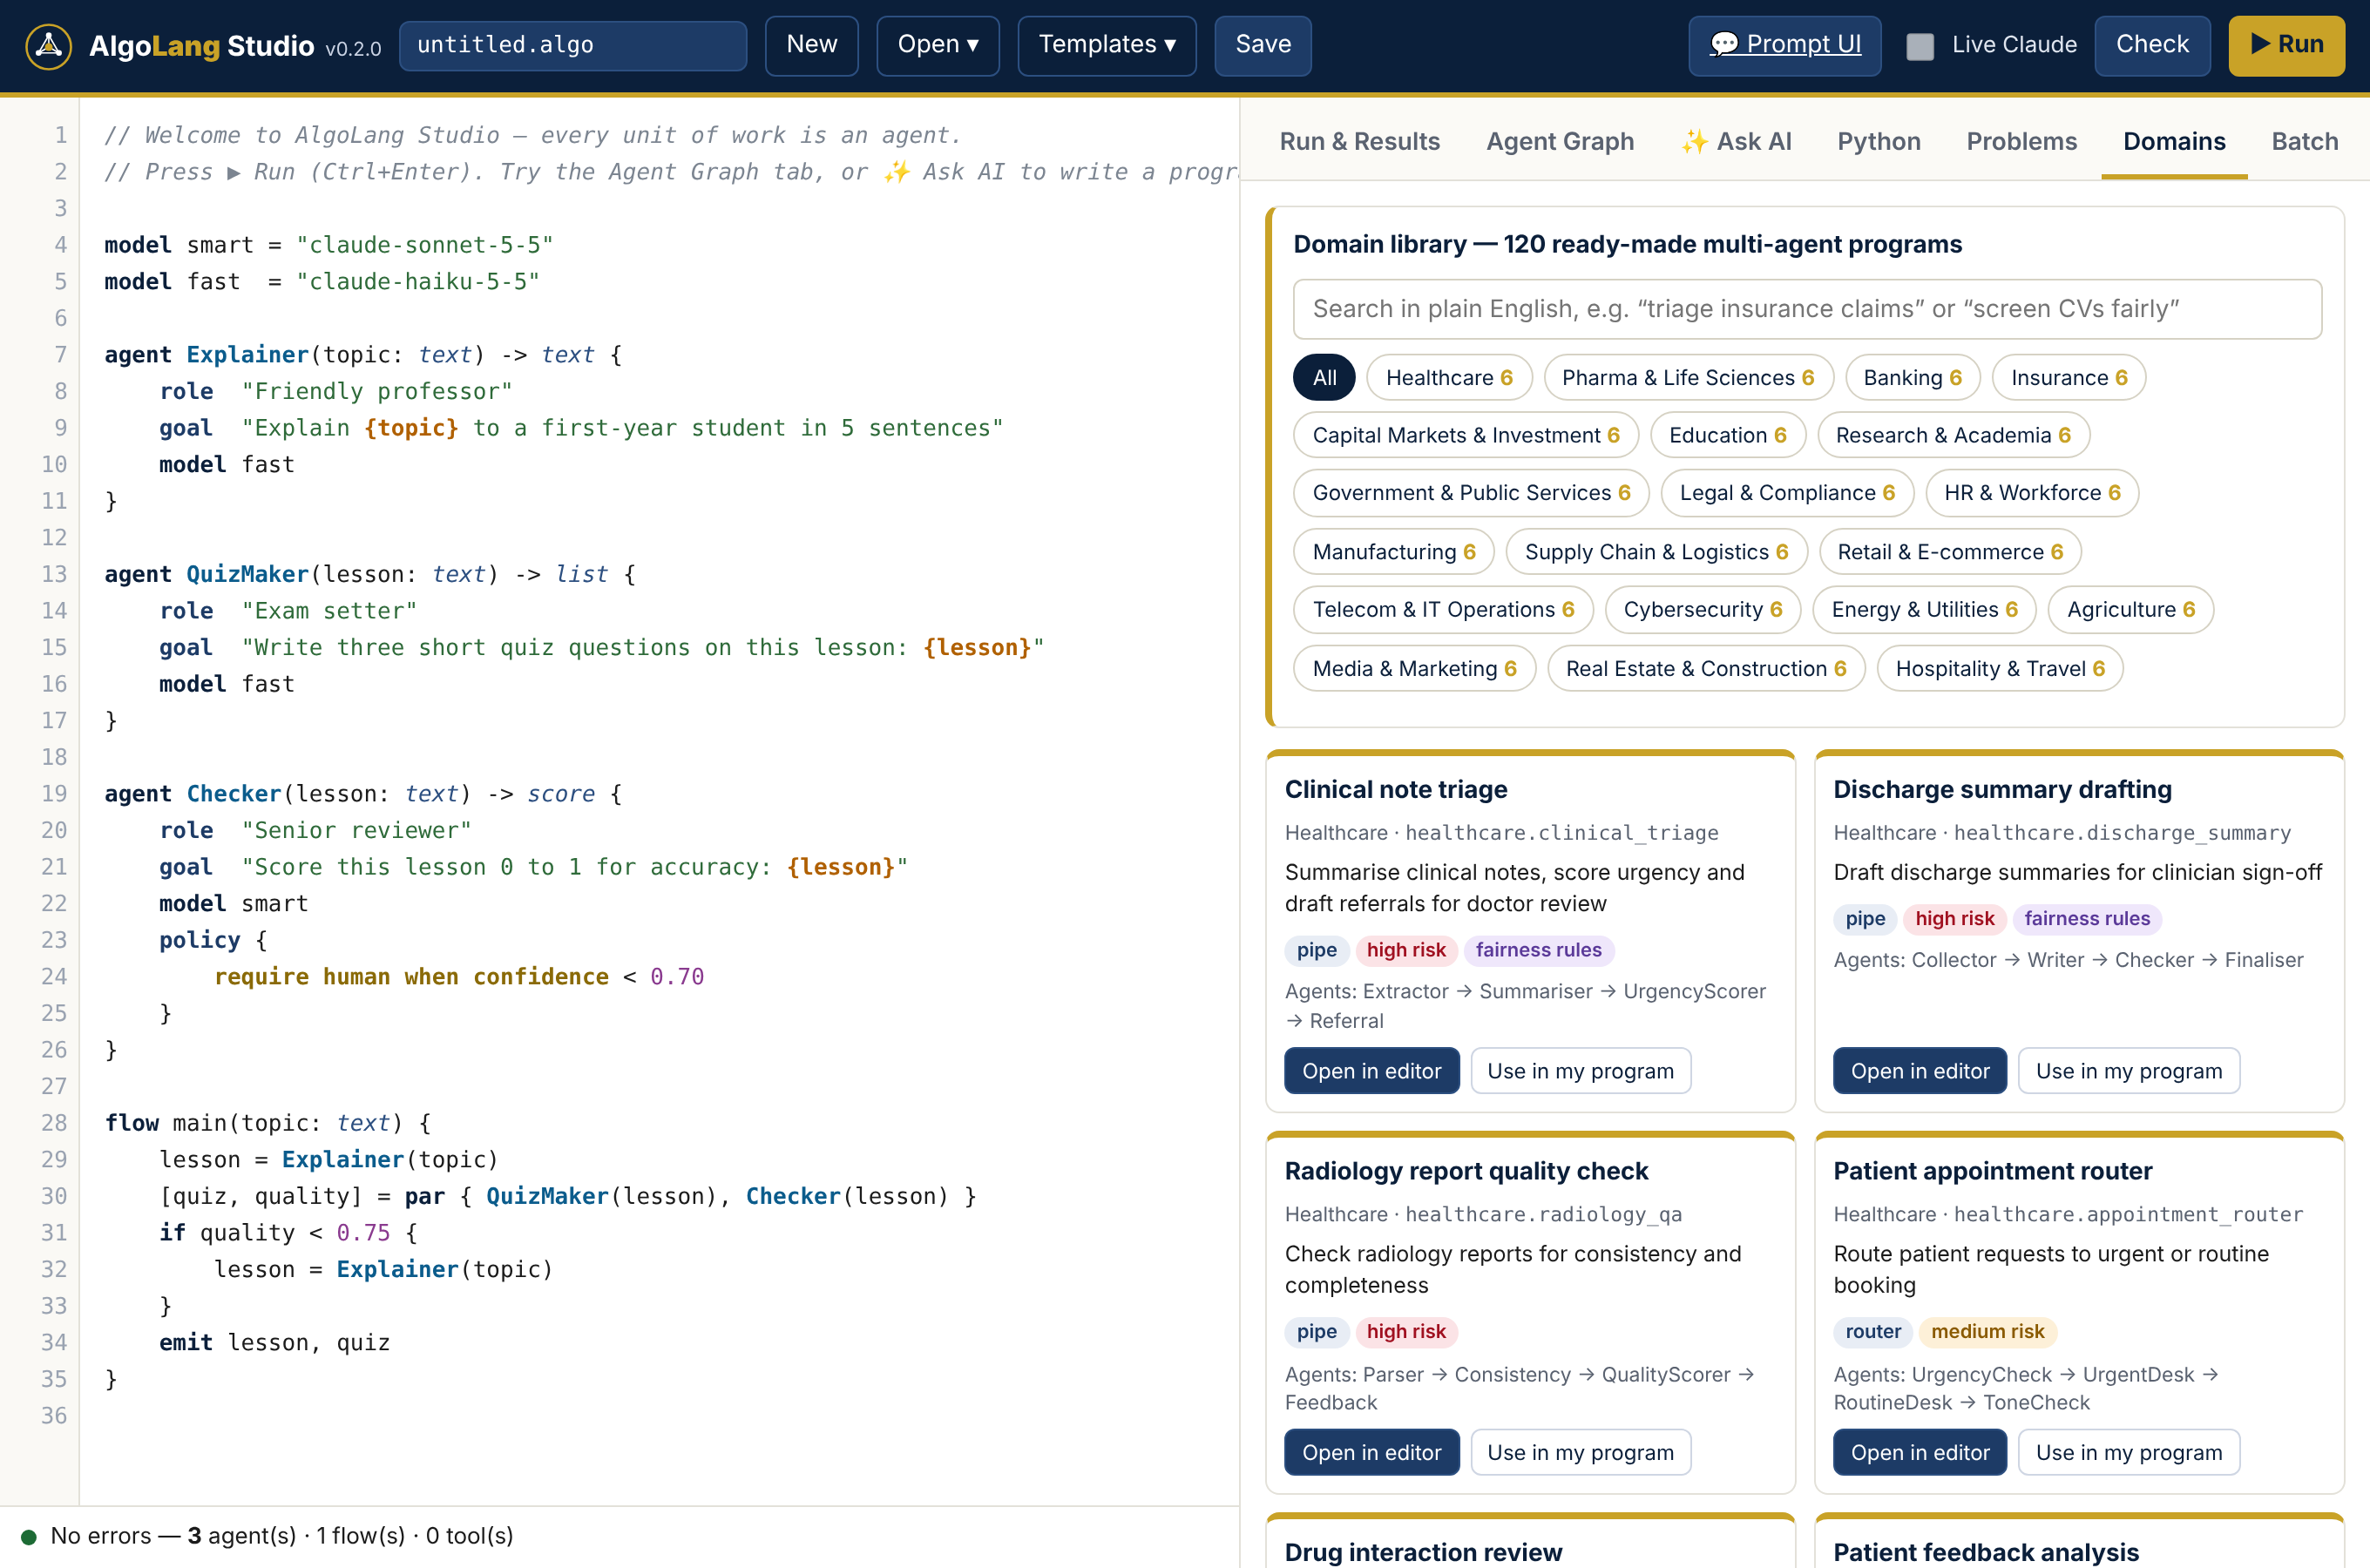
\includegraphics[width=\linewidth]{images/studio-domains.png}
\caption{Studio's Domains tab: 120 packs grouped by sector, each showing its pattern, risk level and agents.}
\label{fig:studiodomains}
\end{figure}

\begin{figure}[ht]
\centering
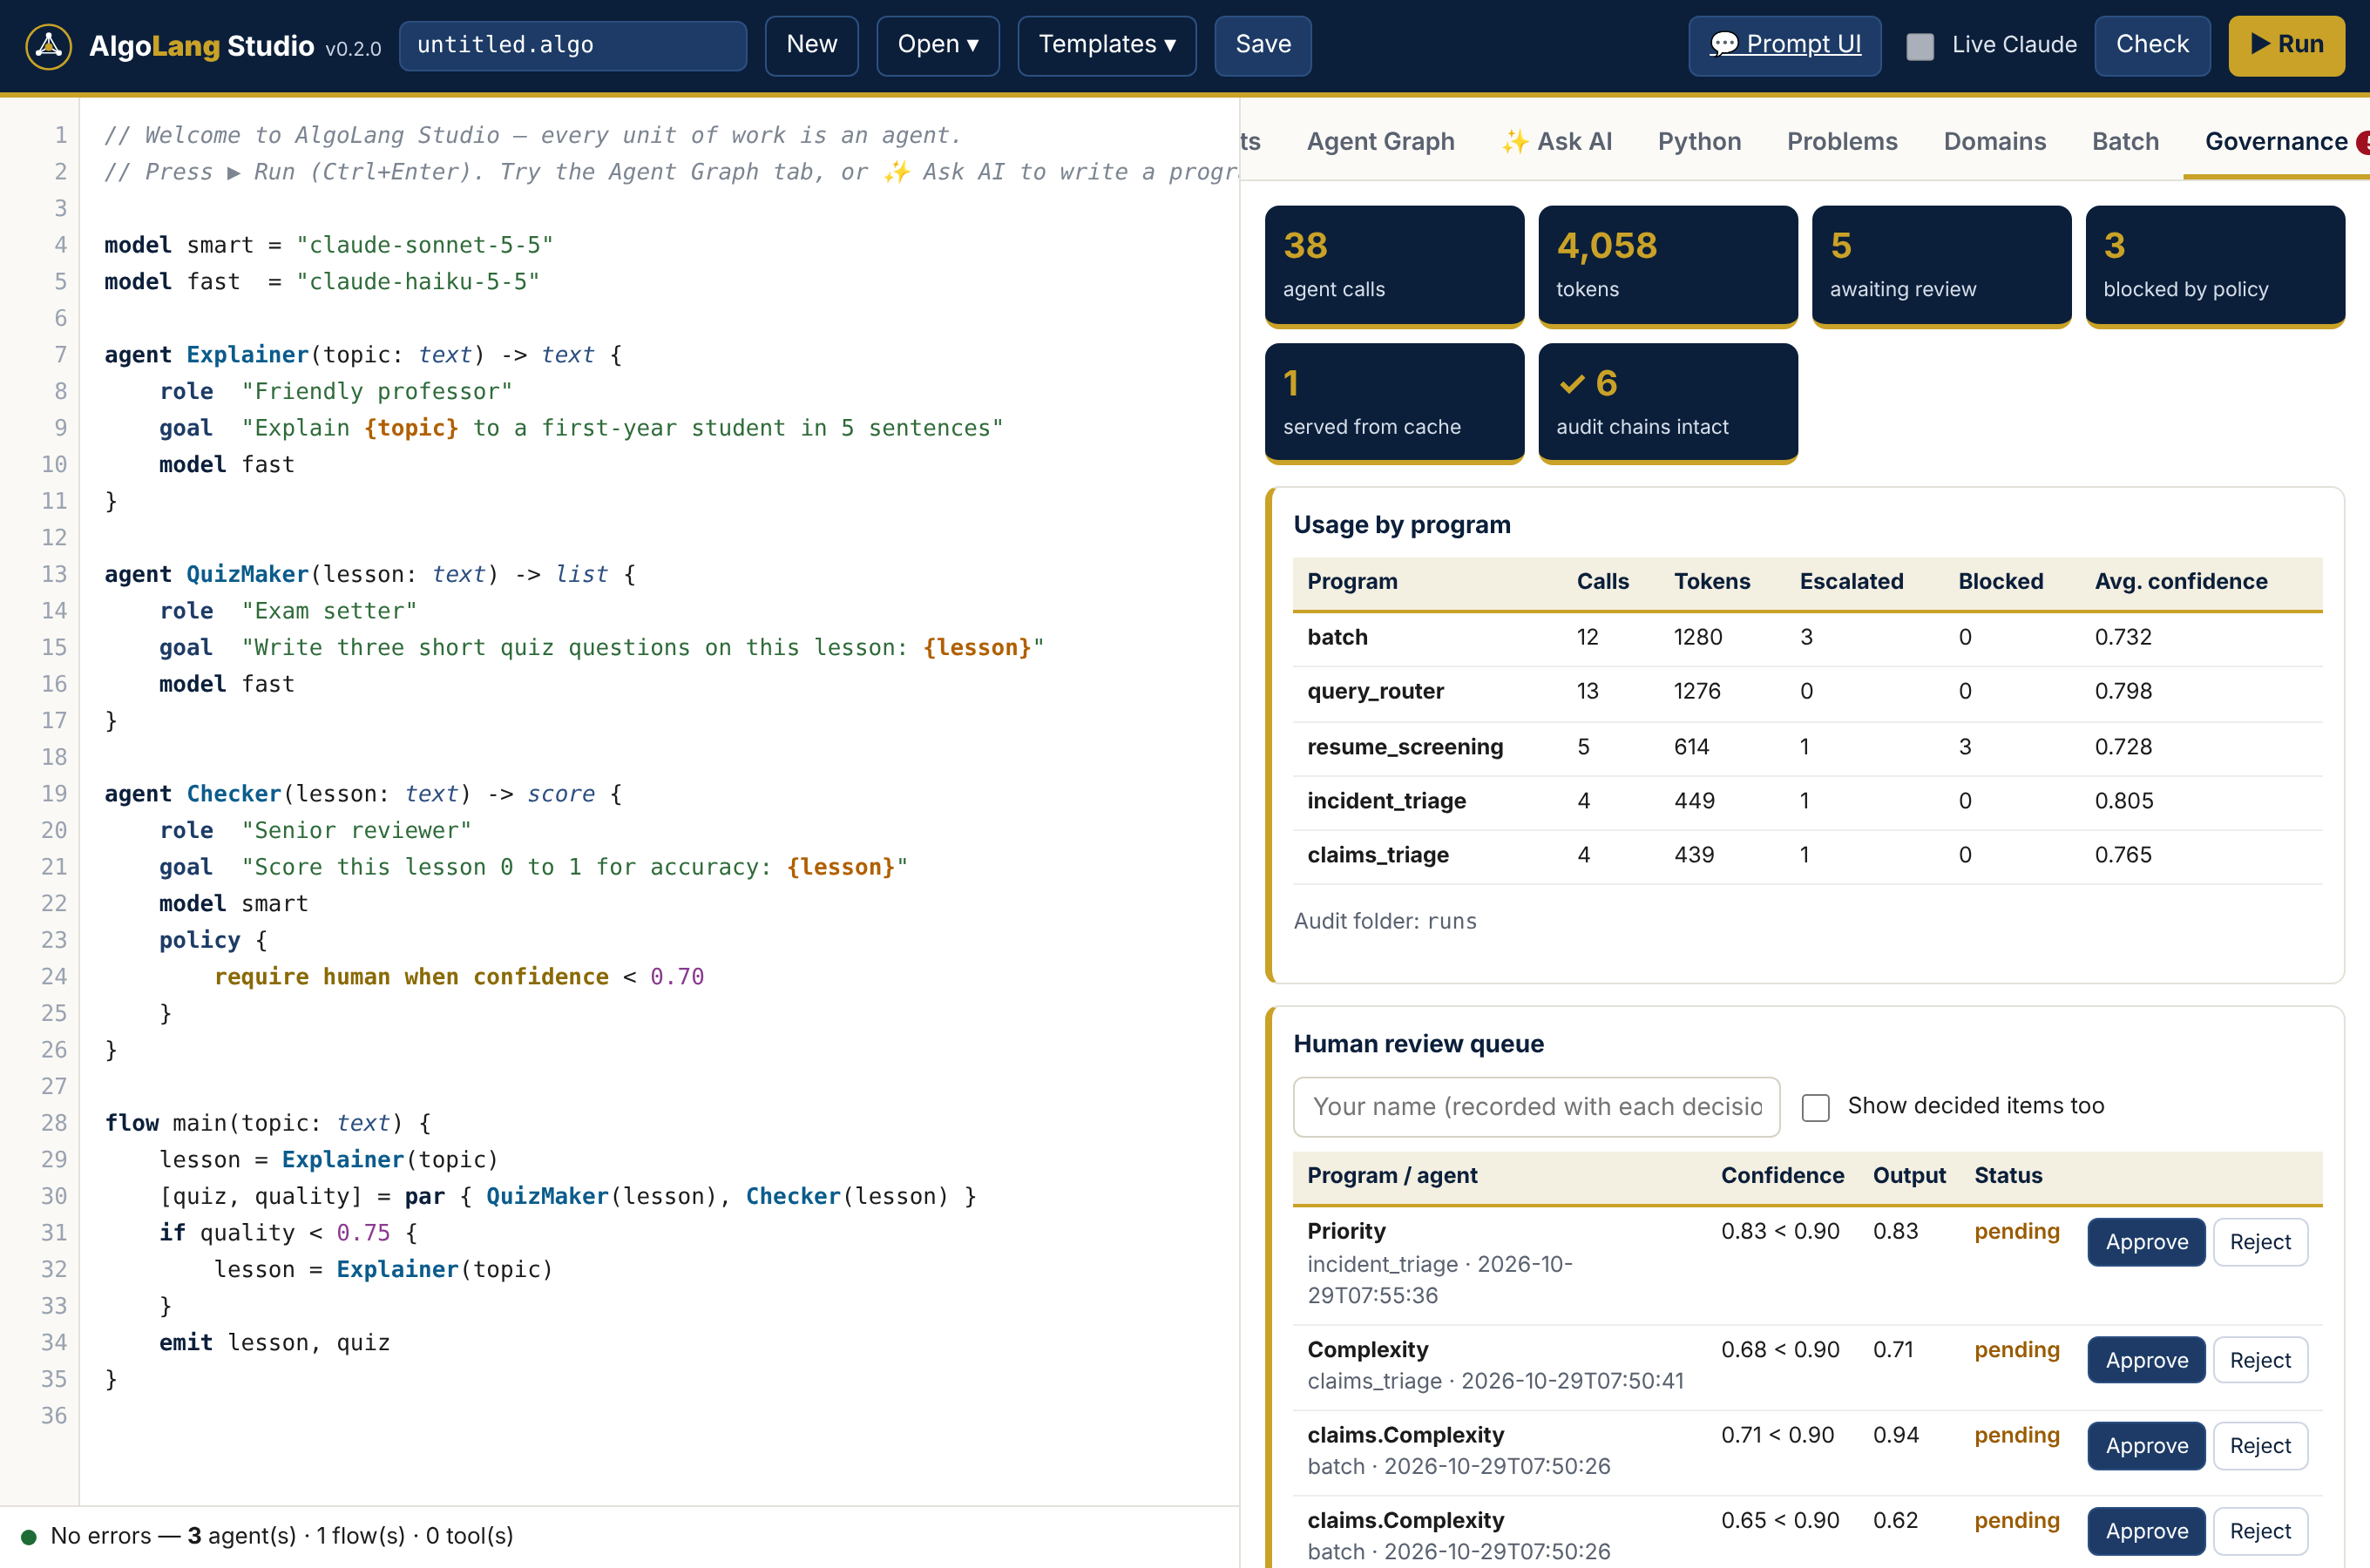
\includegraphics[width=\linewidth]{images/studio-governance.png}
\caption{Studio's Governance tab: usage and audit-chain tiles, usage per program, and the human review queue.}
\label{fig:studiogov}
\end{figure}

\subsection{Mode 3: Prompt-based UI}

\code{algo ui} opens a chat-style page for people who will never open an editor. They describe the problem in plain English. \algolang\ picks the best domain program, runs it under the org policy, and shows:
\begin{itemize}
\item the chain of agents;
\item the governance applied;
\item the result and any items waiting for human review;
\item a table of what each agent did;
\item the program source.
\end{itemize}
Alternatives are one click away. \emph{Open in Studio} hands the program to the graphical mode, and \emph{Customise with AI} asks Claude to adapt it (live mode).

\begin{figure}[ht]
\centering
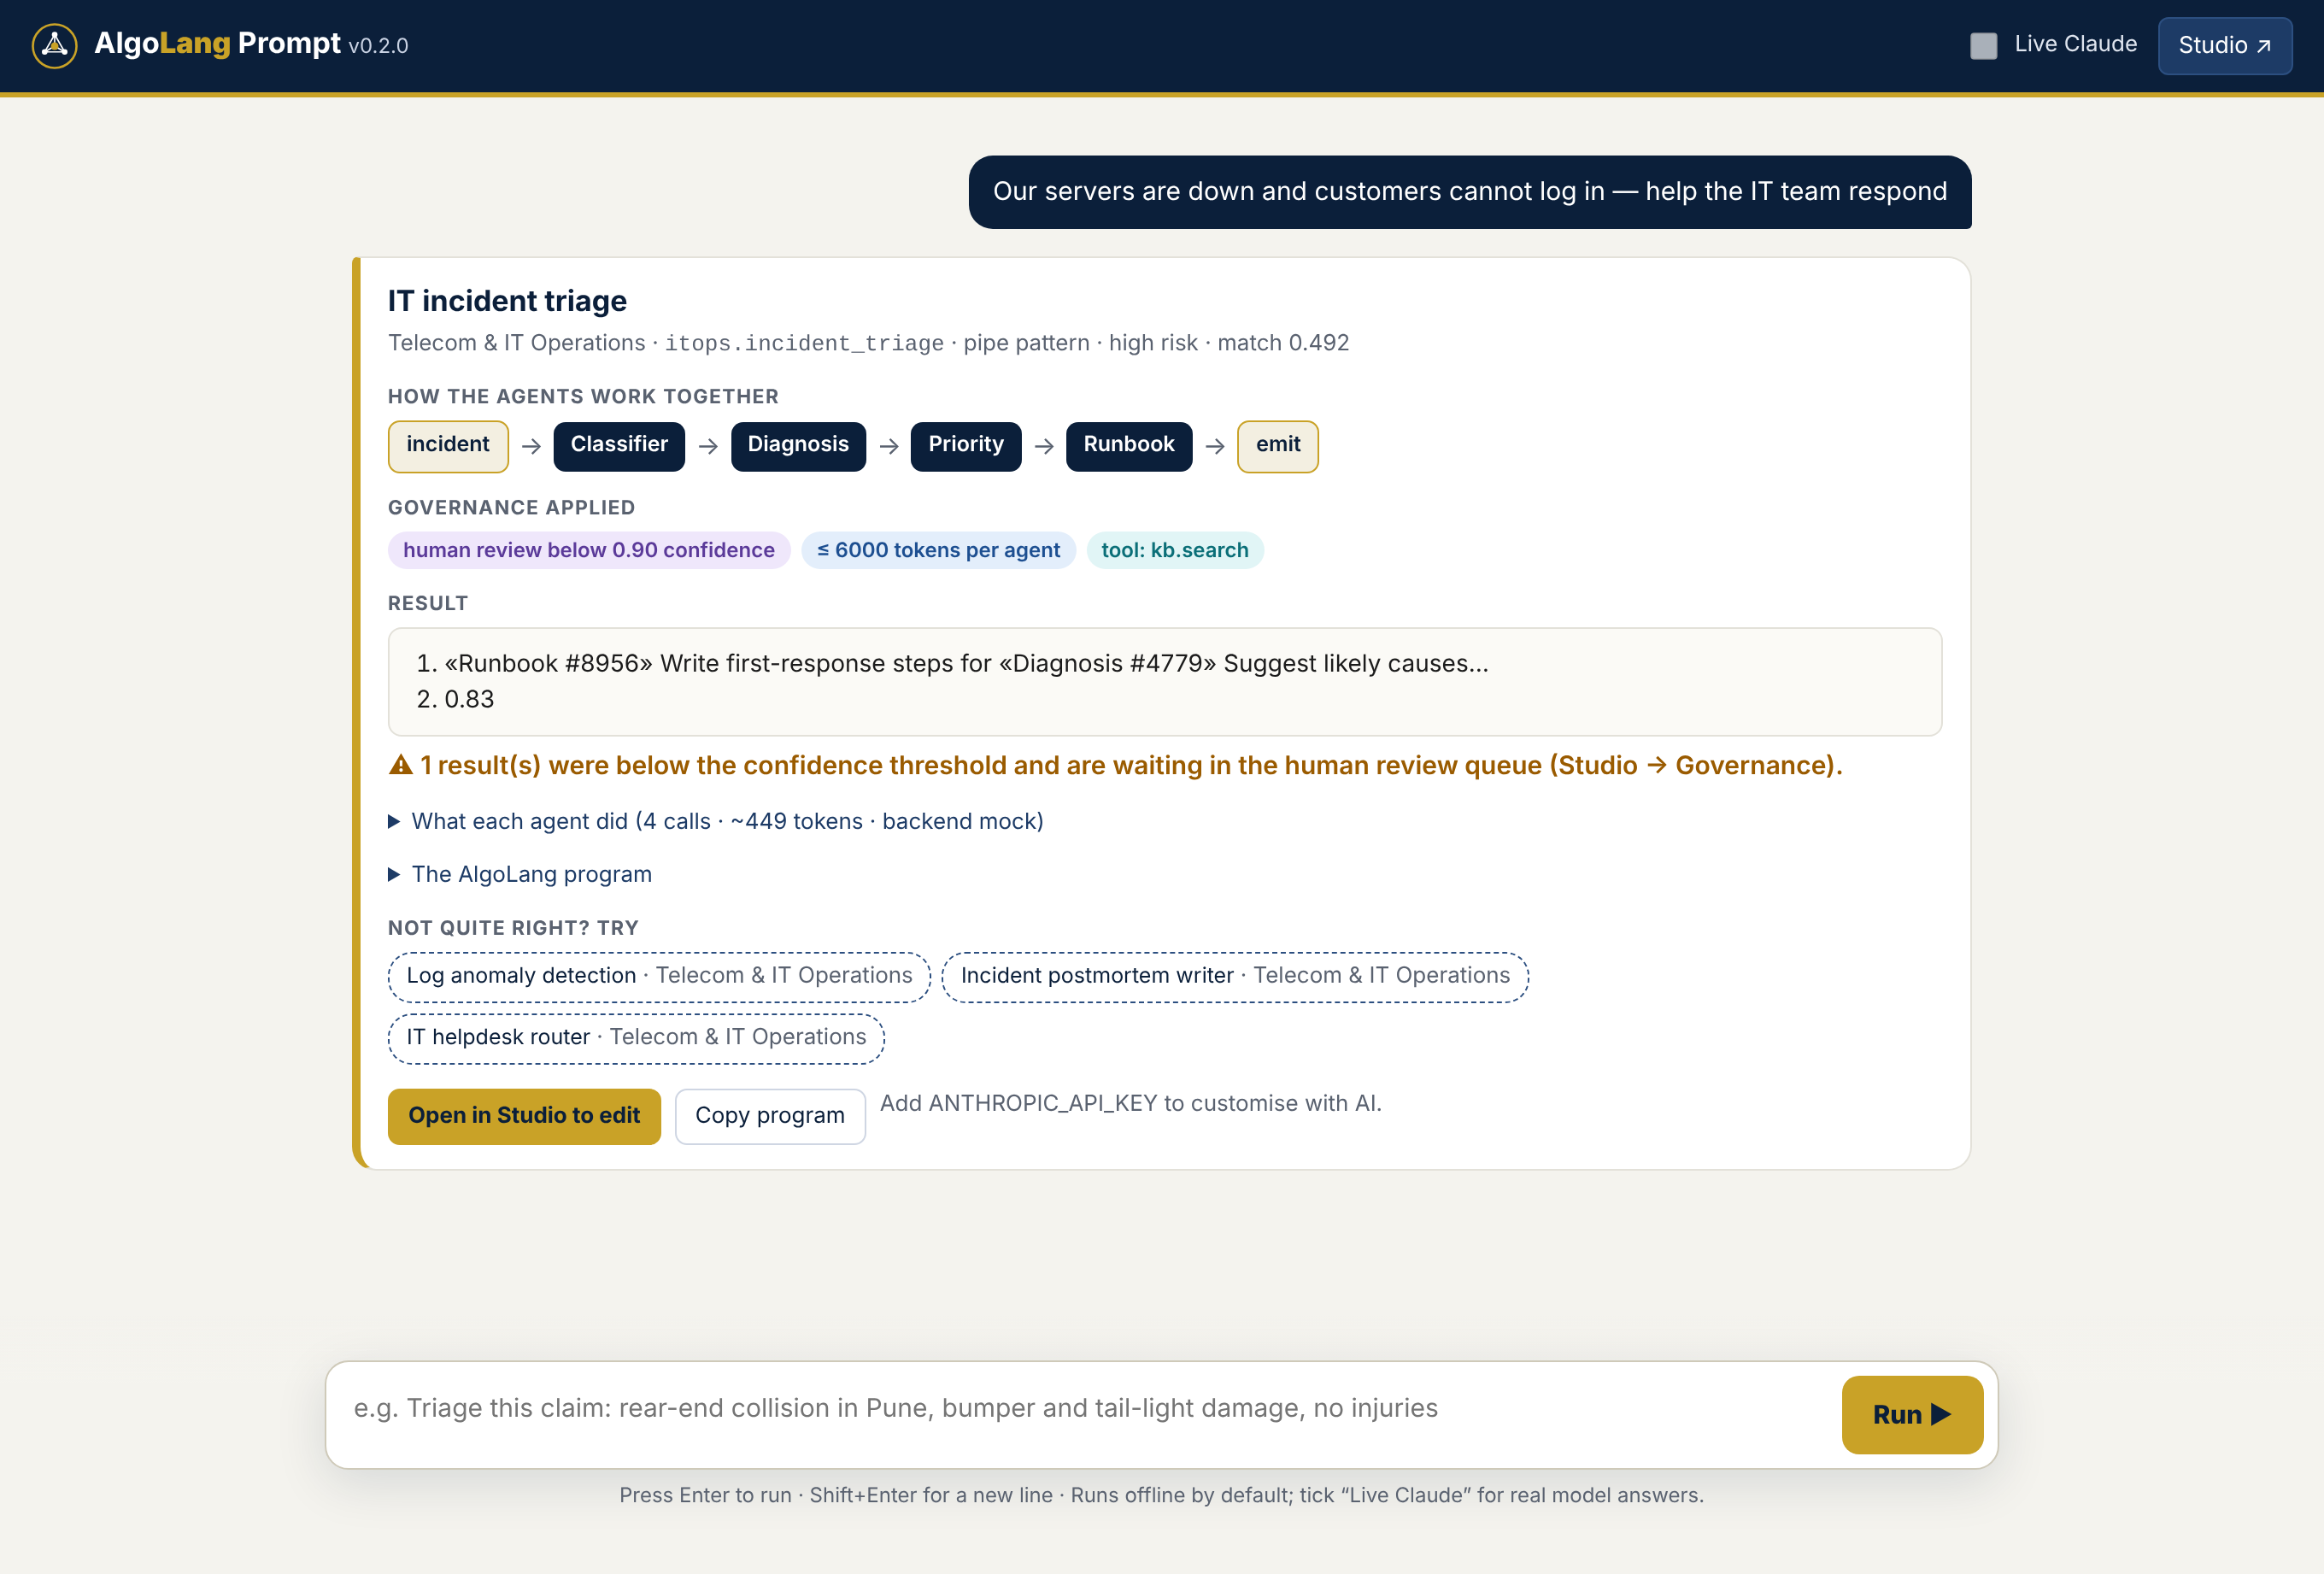
\includegraphics[width=\linewidth]{images/prompt-answer.png}
\caption{The Prompt UI answering an IT outage request with the \code{itops.incident\_triage} pack.}
\label{fig:promptui}
\end{figure}

\begin{ethics}
Governance in \algolang\ is enforced by the compiler and runtime. It is not left to good intentions. Forbidden attributes cannot reach an agent, low-confidence results wait for a named human, and any attempt to rewrite the audit trail is detected. Organisations should still review each domain pack before production use. The packs are well-governed starting points, not certified decision systems.
\end{ethics}


\docpart{Patterns and Practice}
\chapter{Multi-Agent Design Patterns}
\label{ch:patterns}

Good multi-agent systems are built from a small number of recurring shapes. This chapter gives each pattern in \algolang, with guidance on when to use it. All snippets assume suitable agent declarations.

\section{Pipeline}

Each agent refines the previous agent's output.

\begin{algo}
flow main(topic: text) {
    facts   = Researcher(topic)
    outline = Outliner(facts)
    draft   = Writer(outline)
    final   = Editor(draft)
    emit final
}
\end{algo}

\textbf{Use when} the work has clear stages with different skills. \textbf{Tip:} give later, cheaper stages a \code{fast} model and reserve \code{smart} for the stage that needs judgement.

\section{Fan-out / fan-in}

A planner splits the work, one worker per part runs in parallel, and an aggregator combines the results.

\begin{algo}
flow main(paper: text) {
    criteria = Planner(paper)                                       // fan-out plan
    reports  = par for c in criteria { CriterionReviewer(c, paper) } // parallel workers
    summary  = Synthesiser(reports)                                  // fan-in
    emit summary
}
\end{algo}

\textbf{Use when} a task decomposes into independent parts. Total time is roughly that of the slowest worker, not the sum of all workers.

\section{Committee}

Several agents with different perspectives answer the same question; a judge weighs their answers.

\begin{algo}
flow main(question: text) {
    [clinician, statistician, ethicist] = par {
        ClinicalExpert(question), StatsExpert(question), EthicsExpert(question)
    }
    verdict = Judge(clinician, statistician, ethicist)
    emit verdict
}
\end{algo}

\textbf{Use when} decisions benefit from diverse viewpoints, or to reduce the errors of any single agent. Give the members different roles, and if possible different models.

\section{Critic and revise}

A generator drafts, a critic scores, and the generator revises when the score is low.

\begin{algo}
flow main(brief: text) {
    draft = Writer(brief)
    if Critic(draft) < 0.8 {
        draft = Writer(brief, tone = "more rigorous, address the critic's points")
    }
    if Critic(draft) < 0.8 {
        draft = Writer(brief, tone = "concise and fully referenced")
    }
    emit draft
}
\end{algo}

\begin{note}
\algolang\ has no unbounded loops. Revision rounds are written out, so every program is guaranteed to finish and its maximum number of agent calls---and therefore its maximum cost---can be read from the source. This is a deliberate design choice, not an omission.
\end{note}

\section{Router}

A classifier agent decides which specialist handles the input.

\begin{algo}
flow main(query: text) {
    technical = IsTechnical(query)          // returns score
    if technical >= 0.5 {
        answer = TechSupport(query)
    } else {
        answer = GeneralHelp(query)
    }
    emit answer
}
\end{algo}

\section{Guardrail}

A checking agent screens input before the main work begins.

\begin{algo}
agent SafetyCheck(request: text) -> bool {
    role "Safety reviewer"
    goal "Answer true only if this request is safe and appropriate to fulfil: {request}"
}

flow main(request: text) {
    safe = SafetyCheck(request)
    if safe == true {
        emit Assistant(request)
    } else {
        emit Refusal(request)
    }
}
\end{algo}

\section{Human-in-the-loop}

Place a confidence gate on the agent whose output matters most, and run with \code{--interactive} where a person is present.

\begin{algo}
agent Grader(answer: text, rubric: text) -> score {
    role  "Examiner"
    goal  "Grade {answer} against {rubric}; 0 to 1"
    policy { require human when confidence < 0.85 }
}
\end{algo}

\section{Separation of duties}

The agent that \emph{decides} must not be the agent that \emph{audits}. Keep them separate, with separate policies.

\begin{algo}
agent Decider(application: text) -> score {
    goal   "Score {application} for the scholarship criteria only"
    policy { forbid gender, caste, religion  require human when confidence < 0.8 }
}

agent FairnessAuditor(decisions: list) -> text {
    role "Independent fairness auditor"
    goal "Review {decisions} for patterns of unfair treatment and explain any concerns"
}
\end{algo}

\begin{ethics}[Why separation matters]
An agent asked to both decide and justify its own fairness has a conflict of interest, just as a person would. Separate agents make the audit independent, appear as separate entries in the audit log, and can be given different models and different reviewers.
\end{ethics}

\section{Choosing a pattern}

\begin{center}
\small
\begin{tabularx}{\linewidth}{@{}L{3.6cm}Y@{}}
\toprule
\thead{If you need…} & \thead{Use}\\
\goldrule
Stages with different skills & Pipeline\\
Speed on decomposable work & Fan-out / fan-in\\
Robust decisions & Committee\\
Higher quality output & Critic and revise\\
Different handling per input & Router\\
Safety before work begins & Guardrail\\
Accountable decisions about people & Human-in-the-loop + separation of duties\\
\bottomrule
\end{tabularx}
\end{center}

\chapter{Responsible AI with AlgoLang}
\label{ch:responsible}

\algolang\ was designed so that the responsible way to build an AI system is also the easiest way. This chapter maps its features to widely used principles of trustworthy AI, shows how to use them together, and states plainly what the language does \emph{not} guarantee.

\section{Principles and features}

\begin{center}
\small
\begin{tabularx}{\linewidth}{@{}L{3.2cm}YL{3.6cm}@{}}
\toprule
\thead{Principle} & \thead{How AlgoLang supports it} & \thead{Feature}\\
\goldrule
Accountability & Every unit of work is named and has a stated goal; every call is recorded & agents only (\errcode{E101}); audit log\\
Human oversight & Low-confidence results are routed to people; reviewers can approve & \kw{require human when}; \code{--interactive}\\
Fairness & Protected attributes cannot be declared as inputs and are blocked in prompts & \kw{forbid} (\errcode{E108}, run-time block)\\
Transparency & Capabilities, models and policies are visible in the source and in each audit record & \kw{tool}, \kw{uses}, \kw{model}, \kw{policy}\\
Security & Agents receive only explicitly granted capabilities & declared tools (\errcode{E104})\\
Privacy & The log stores prompt hashes, not prompts or outputs & \code{inputs\_sha}\\
Sustainability \& cost & Per-agent token budgets; bounded programs with no unbounded loops & \kw{budget tokens}; flow design\\
Reliability & Retries, timeouts; deterministic offline testing & \kw{retry}, \kw{timeout}; mock backend\\
\bottomrule
\end{tabularx}
\end{center}

\section{Supporting governance frameworks}

Organisations increasingly align AI systems with frameworks such as the NIST AI Risk Management Framework (with its functions \emph{Govern}, \emph{Map}, \emph{Measure} and \emph{Manage}) and, in Europe, the AI Act's requirements for high-risk systems, which include record-keeping (Article~12) and human oversight (Article~14). \algolang\ does not make a system compliant with any framework---compliance depends on the whole system and its context---but its features produce evidence that such work needs:

\begin{itemize}
  \item the \textbf{source program} documents what each agent does, with which model and capabilities, under which rules;
  \item the \textbf{audit log} records every call, its confidence and its outcome;
  \item \textbf{escalation counts} and \textbf{approvals} show where human oversight was exercised;
  \item \textbf{blocked calls} show where safeguards acted.
\end{itemize}

\section{A responsible design checklist}

\begin{enumerate}
  \item Does every agent have one clear goal and the narrowest return type?
  \item Does each agent hold only the tools it needs?
  \item Do agents that affect people have a human-review threshold, chosen deliberately?
  \item Are protected attributes listed in \kw{forbid} for every decision-making agent?
  \item Is auditing done by a separate agent from deciding?
  \item Does every live agent have a token budget?
  \item Have you run the program on the mock backend and read the audit log before going live?
  \item Who reviews escalated results, how quickly, and where is that recorded?
  \item Have you tested outcomes across groups, not only individual cases?
\end{enumerate}

\section{Known limitations}
\label{sec:limits}

Version 0.1 is a preview. The following limitations are known and documented so that no one relies on a guarantee the language does not give.

\begin{center}
\small
\begin{tabularx}{\linewidth}{@{}L{3.4cm}Y@{}}
\toprule
\thead{Area} & \thead{Limitation in v0.1}\\
\goldrule
\kw{forbid} & Lexical: blocks the forbidden words, not proxies (names, places, schools) that may reveal the same attribute. Not a fairness guarantee.\\
Confidence (live) & Reported by the model itself. It is not a calibrated probability and should be validated against real outcomes before thresholds are trusted.\\
Confidence (mock) & Synthetic, derived from a hash of the input; useful only for demonstrating behaviour.\\
Token budget & Estimated at about four characters per token before the call; real counts may differ.\\
Timeout & Checked when the call returns; a slow call is not interrupted.\\
Tools & Declared and enforced as capabilities, but not executed by the runtime yet.\\
Types & Argument types are not yet checked against parameter types; flow inputs arrive as text.\\
Prompt injection & Text inside inputs can try to steer an agent. Policies limit what an agent may do, but do not detect injected instructions.\\
Audit log & Local append-only file; it is not tamper-proof. Protect and back it up as you would any record.\\
\bottomrule
\end{tabularx}
\end{center}

\begin{caution}[Use with care]
Do not use \algolang~0.1 as the sole basis for decisions with legal or similarly significant effects on people---admissions, hiring, credit, health or justice---without independent validation, human review of every decision, and the governance your institution and law require.
\end{caution}

\section{Teaching AI ethics with AlgoLang}

Because policies are code, ethical questions become concrete design exercises that students can run, break and discuss:

\begin{itemize}
  \item \textbf{Proxy discrimination.} Build a screening flow that forbids \code{caste}, then show that a surname or home-district input can still carry the same information. Discuss what \kw{forbid} can and cannot do.
  \item \textbf{Automation bias.} Run with \code{--interactive} and track how often reviewers approve without reading. Discuss how to design review that is meaningful.
  \item \textbf{Threshold setting.} Vary \kw{require human} thresholds and measure escalation rates. Who should choose the threshold, and how should it be justified?
  \item \textbf{Accountability.} Given only an audit log, reconstruct what happened in a run. What is missing that a regulator or an affected person would need?
\end{itemize}

\chapter{Teaching with AlgoLang}
\label{ch:teaching}

\algolang\ is small enough to learn in one session and rich enough to support a full course module on agentic AI and responsible AI. The mock backend makes every lab free, repeatable and runnable offline; Google Colab removes installation entirely.

\section{Suggested lab sequence}

\begin{center}
\small
\begin{tabularx}{\linewidth}{@{}L{0.7cm}L{3.6cm}YL{2.4cm}@{}}
\toprule
\thead{Lab} & \thead{Topic} & \thead{Students build} & \thead{Concepts}\\
\goldrule
1 & First agents & The starter program from \code{algo new}; change goals and roles & agent, goal, flow\\
2 & Types and scores & A grader that returns a \kw{score} and a branch on it & types, \kw{if}, \errcode{E110}\\
3 & Reading errors & Fix a broken program with eight errors & compiler diagnostics\\
4 & Parallel agents & A committee of three experts and a judge & \kw{par}\\
5 & Planning & A planner and \kw{par for} workers & fan-out / fan-in\\
6 & Capabilities & Grant and remove tools; observe \errcode{E104} & least privilege\\
7 & Human oversight & Gate a decision agent; run with \code{--interactive} & oversight, thresholds\\
8 & Fairness & A screening flow with \kw{forbid}; probe it with proxy attributes & fairness limits\\
9 & Audit & Load the audit log into \code{pandas}; reconstruct a run & accountability\\
10 & Going live & Run a finished flow on Claude with budgets & cost, real outputs\\
\bottomrule
\end{tabularx}
\end{center}

\section{Exercises}

\begin{enumerate}
  \item \textbf{Translator.} Add \code{Translator(passage: text, language: text) -> text} and produce Hindi and Marathi versions of a brief in one \kw{par} block.
  \item \textbf{Budget discipline.} Give \code{Writer} the policy \code{budget tokens 50} and run. Explain the outcome and why it is better to fail before a call than to discover the cost afterwards.
  \item \textbf{Committee size.} Extend a committee from three to five experts. How does run time change on the mock backend, and why?
  \item \textbf{Bounded revision.} Write a critic-and-revise flow with at most three revisions. What is the maximum number of agent calls? Prove it from the source.
  \item \textbf{Scholarship screening.} Design a flow that scores applications without seeing gender or caste, sends uncertain cases to a human, and has a separate fairness auditor. Then try to break it.
  \item \textbf{Audit questions.} From an audit log alone, answer: which agent was least confident on average? How many results were escalated? Which model handled which agent?
  \item \textbf{Language design.} Propose a new policy rule (for example, a maximum number of calls per agent). Write the grammar change and describe the runtime check (Chapter~\ref{ch:internals}).
\end{enumerate}

\section{Assessment ideas}

\begin{center}
\small
\begin{tabularx}{\linewidth}{@{}L{3.6cm}Y@{}}
\toprule
\thead{Criterion} & \thead{Evidence}\\
\goldrule
Correctness & Program compiles with no errors and produces the required outputs\\
Decomposition & Agents have single, clear goals and appropriate return types\\
Use of patterns & Parallelism and branching are used where they fit\\
Governance & Budgets, human-review thresholds and forbidden attributes are present and justified in writing\\
Evidence & Audit log analysed; escalations and blocks explained\\
Reflection & A short essay on one limitation from Section~\ref{sec:limits} and how to mitigate it\\
\bottomrule
\end{tabularx}
\end{center}

\section{Using the notebook in class}

Share \file{AlgoLang\_Notebook.ipynb} with students; each opens it in their own Colab session. The notebook's ten sections follow the order of this book and end with exercises. Students can edit the toolchain cells themselves, which makes the notebook suitable for compiler-construction and programming-languages courses as well as AI courses.


\docpart{The Project}
\chapter{The AlgoLang Project}
\label{ch:project}

\algolang\ is an open-source project led by AlgoProfessor AI R\&D Solutions. This chapter describes how the project is organised, where it is going and how you can take part.

\section{Versioning}

\algolang\ follows semantic versioning. During the 0.x series, minor versions (0.2, 0.3, …) may change the language; patch versions (0.1.1, …) fix defects without changing valid programs. From version 1.0, any program that compiles under 1.$x$ will compile under every later 1.$y$.

\section{Roadmap}

\begin{figure}[ht]
\centering
\begin{tikzpicture}[
  ms/.style={circle,fill=gold,draw=navy,line width=1pt,minimum size=4mm,inner sep=0pt},
  now/.style={ms,fill=navy},
  lab/.style={font=\sffamily\bfseries\small,text=navy,anchor=south},
  txt/.style={font=\sffamily\scriptsize,text=ink,align=left,anchor=north,text width=36mm}]
  \draw[navy,line width=1.6pt] (0.2,0) -- (15.3,0);
  \node[ms] at (1.9,0) {};  \node[lab] at (1.9,0.3)  {v0.1};
  \node[now] at (6.0,0) {};  \node[lab] at (6.0,0.3)  {v0.2 · now};
  \node[ms]  at (10.1,0) {}; \node[lab] at (10.1,0.3) {v0.3};
  \node[ms]  at (14.0,0) {}; \node[lab] at (14.0,0.3) {v1.0};
  \node[txt] at (1.9,-0.35)  {Agents, flows, policies\\ par / par for\\ mock + live backends\\ audit log, notebooks};
  \node[txt] at (6.0,-0.35)  {Enterprise: modules, org policy\\ 120 domain packs\\ executable tools, batch\\ hash-chained audit, review\\ SDK + Prompt UI};
  \node[txt] at (10.1,-0.35) {\texttt{uncertain<T>}, type checks\\ \texttt{eval} + trace replay\\ MCP bindings, LSP\\ cost and energy budgets};
  \node[txt] at (14.0,-0.35) {Stable language\\ typed agent messaging\\ native runtime\\ package registry};
\end{tikzpicture}
\caption{Roadmap. Dates are not fixed; each step ships when its features are complete and documented.}
\end{figure}

\section{Proposing changes: AEPs}

Significant changes to the language are made through \textbf{AlgoLang Enhancement Proposals (AEPs)}, short design documents in the tradition of other open-source languages.

\begin{enumerate}
  \item \textbf{Discuss} the idea informally first.
  \item \textbf{Write an AEP} with: motivation; the proposed syntax and semantics; examples; effect on existing programs; implementation sketch (grammar, checker, runtime); and the responsible-AI implications of the change.
  \item \textbf{Review.} Proposals are reviewed for clarity, consistency with the design goals in Chapter~\ref{ch:intro}, and the impact on accountability and safety.
  \item \textbf{Decide.} Accepted AEPs are numbered, implemented with tests and documentation, and listed in the release notes.
\end{enumerate}

\begin{ethics}[A required section]
Every AEP must include a section on responsible-AI implications. A feature that makes AI work less visible, less accountable or harder to oversee needs a strong justification and compensating safeguards.
\end{ethics}

\section{Contributing}

Contributions of every size are welcome:

\begin{itemize}
  \item \textbf{Report a problem:} include the \file{.algo} file, the exact command, the full output and the output of \code{algo doctor}.
  \item \textbf{Improve documentation or examples:} new examples, teaching material and translations are especially valuable.
  \item \textbf{Change the code:} keep the compiler and runtime small and readable; add an example that exercises the change; run every example with \code{algo check} and \code{algo run} on the mock backend before submitting.
\end{itemize}

Contact: \href{mailto:ceo@algoprofessor.com}{ceo@algoprofessor.com} · \href{https://www.algoprofessor.com}{www.algoprofessor.com}.

\section{Code of conduct}

The \algolang\ community is open to everyone. Participants are expected to be respectful and constructive, to welcome newcomers and students, to give credit, and to assume good faith. Harassment and discrimination of any kind are not tolerated.

\section{Licence}

The \algolang\ software (compiler, runtime, notebook extension, installers and examples) is licensed under the \textbf{Apache License, Version 2.0}. This documentation is licensed under \textbf{Creative Commons Attribution 4.0 International (CC BY 4.0)}.

\section{How to cite AlgoLang}
\label{sec:cite}

If you use \algolang\ in research or teaching, please cite this documentation:

\begin{plaincode}[title=BibTeX,unbreakable]
@manual{satyanarayana2026algolang,
  title        = {The {AlgoLang} Programming Language: Official Documentation, Version 0.1},
  author       = {Satyanarayana, S.},
  organization = {AlgoProfessor AI R\&D Solutions},
  address      = {Hyderabad, India},
  year         = {2026},
  month        = oct,
  url          = {https://www.algoprofessor.com},
  note         = {Open-source, agent-native programming language for building AI systems}
}
\end{plaincode}


\appendix
\appendixmarks
\chapter{Grammar}
\label{app:grammar}

This appendix reproduces \file{grammar.lark}, the normative grammar of \algolang~0.1, in Lark's EBNF notation. Quoted strings are keywords and punctuation; upper-case names are terminals; \code{?rule} inlines a rule with a single child; \code{-> name} labels an alternative in the parse tree; \code{\%ignore} lists text skipped between tokens.

\begin{plaincode}[title=grammar.lark]
// ─────────────────────────────────────────────────────────────
//  AlgoLang v0.1 grammar  —  AlgoProfessor AI R&D Solutions
//  Core rule: there are no functions. Every unit of work is an
//  `agent`; a `flow` only orchestrates agents.
// ─────────────────────────────────────────────────────────────

start: item*

?item: model_decl
     | tool_decl
     | agent_decl
     | flow_decl

// model fast = "claude-haiku-5-5"
model_decl: "model" NAME "=" STRING

// tool web.search   (declares a tool agents may be granted)
tool_decl: "tool" DOTTED

// agent Name(p: type, q: type = "x") -> type { ... }
agent_decl: "agent" NAME "(" [params] ")" "->" NAME "{" agent_clause* "}"

params: param ("," param)*
param: NAME ":" NAME ["=" literal]

?agent_clause: "role" STRING            -> role
             | "goal" STRING            -> goal
             | "uses" DOTTED ("," DOTTED)* -> uses
             | "model" NAME             -> model_ref
             | "policy" "{" policy_rule* "}" -> policy

?policy_rule: "budget" "tokens" NUMBER                       -> budget
            | "retry" NUMBER                                 -> retry
            | "require" "human" "when" "confidence" "<" NUMBER -> human_gate
            | "forbid" NAME ("," NAME)*                      -> forbid
            | "timeout" NUMBER                               -> timeout

// flow main(topic: text) { ... }
flow_decl: "flow" NAME "(" [params] ")" "{" stmt* "}"

?stmt: target "=" expr                                   -> assign
     | "if" cond "{" stmt* "}" ["else" "{" stmt* "}"]    -> if_stmt
     | "emit" expr ("," expr)*                           -> emit
     | call                                              -> expr_stmt

target: NAME                         -> single_target
      | "[" NAME ("," NAME)* "]"     -> multi_target

?expr: call
     | par_block
     | par_for
     | NAME                          -> var
     | literal

call: NAME "(" [args] ")"
args: arg ("," arg)*
?arg: kwarg | expr
kwarg: NAME "=" expr

// [a, b] = par { Writer(x), Critic(x) }
par_block: "par" "{" call ("," call)* "}"

// results = par for t in tasks { Worker(t) }
par_for: "par" "for" NAME "in" NAME "{" call "}"

cond: expr COMPARE expr
COMPARE: "<=" | ">=" | "==" | "!=" | "<" | ">"

?literal: STRING -> string
        | NUMBER -> number
        | "true"  -> true
        | "false" -> false

DOTTED: /[a-zA-Z_][a-zA-Z0-9_]*(\.[a-zA-Z_][a-zA-Z0-9_]*)+/
NAME: /[a-zA-Z_][a-zA-Z0-9_]*/
STRING: /"([^"\\]|\\.)*"/
NUMBER: /\d+(\.\d+)?/

COMMENT: /\/\/[^\n]*/
%ignore COMMENT
%import common.WS
%ignore WS
SEMI: ";"
%ignore SEMI
\end{plaincode}

\chapter{Quick Reference}
\label{app:reference}

\section{Language card}

\begin{algo}[title=everything in one screen]
// ── declarations ─────────────────────────────────────────────
model smart = "claude-sonnet-5-5"          // name a model
tool  web.search                            // declare a capability

agent Name(p: text, q: score = 0.5) -> list {   // types: text score list json bool
    role   "who it acts as"
    goal   "what to do with {p} and {q}"         // {param} placeholders
    uses   web.search                            // granted tools
    model  smart
    policy {
        budget tokens 4000                       // stop if prompt larger
        retry 2                                  // retry failures
        timeout 60                               // seconds
        require human when confidence < 0.75     // human oversight
        forbid gender, caste, religion           // protected attributes
    }
}

// ── flow statements ──────────────────────────────────────────
flow main(input: text) {
    x       = Agent(input, q = 0.9)                   // call
    [a, b]  = par { AgentA(x), AgentB(x) }            // parallel block
    rs      = par for item in x { Worker(item) }      // parallel map over list
    if a < 0.8 { b = AgentB(x) } else { b = AgentC(x) }   // branch on score
    Notifier(b)                                        // call for effect
    emit a, rs                                         // output
}
\end{algo}

\section{Error codes}

\begin{center}
\small
\begin{tabularx}{\linewidth}{@{}L{1.3cm}Y L{1.3cm}Y@{}}
\toprule
\thead{Code} & \thead{Meaning} & \thead{Code} & \thead{Meaning}\\
\goldrule
E100 & Syntax error & E108 & Forbidden attribute as parameter\\
E101 & Not an agent & E109 & Unknown \code{\{placeholder\}} in goal\\
E102 & Wrong arguments & E110 & Comparing a non-score\\
E103 & Undefined variable & E111 & No \code{flow main}\\
E104 & Undeclared tool & E112 & Agent without a goal\\
E105 & Unknown type & E113 & \code{[a, b]} does not match \kw{par}\\
E106 & Unknown model & E114 & \kw{par for} over a non-list\\
E107 & Defined twice & E115 & Tool not allowed by org policy\\
\bottomrule
\end{tabularx}
\end{center}

\section{Command line}

\begin{center}
\small
\begin{tabularx}{\linewidth}{@{}L{6.4cm}Y@{}}
\toprule
\thead{Command} & \thead{Purpose}\\
\goldrule
\code{algo doctor} & Check the environment\\
\code{algo new NAME} & Create a starter program\\
\code{algo check F.algo} & Find errors\\
\code{algo build F.algo [-o out.py]} & Compile to Python\\
\code{algo run F.algo --arg "k=v"} & Run on the mock backend\\
\code{  … --live} & Run on Claude\\
\code{  … --interactive} & Approve low-confidence results\\
\code{  … --audit-dir DIR} & Choose where audit logs go\\
\code{algo notebook} & Open the Jupyter notebook\\
\bottomrule
\end{tabularx}
\end{center}

\section{Notebook}

\begin{center}
\small
\begin{tabularx}{\linewidth}{@{}L{6.4cm}Y@{}}
\toprule
\thead{Cell or magic} & \thead{Purpose}\\
\goldrule
\code{\%load\_ext algomagic} & Enable \algolang\ in a notebook\\
\code{\%\%algo --arg "k=v" [--graph] [--python]} & Run the cell\\
\code{\%\%algo --define} & Add declarations to the session\\
\code{\%\%algo --check} & Check only\\
\code{\%algo\_run F.algo --arg "k=v"} & Run a file\\
\code{\%algo\_list}, \code{\%algo\_reset}, \code{\%algo\_help} & Session tools\\
\code{algo\_result}, \code{algo\_calls} & Results for Python cells\\
\bottomrule
\end{tabularx}
\end{center}

\section{Glossary}

\begin{description}[leftmargin=0pt,font=\sffamily\bfseries\color{navy}]
  \item[Agent] A declared unit of work with a goal, optional role, tools, model and policy. The only callable thing in \algolang.
  \item[Audit record] One JSON line per agent call describing what ran, under which rules, with what confidence and outcome.
  \item[Backend] What executes agent calls: \emph{mock} (offline, deterministic) or \emph{live} (Claude models).
  \item[Confidence] A number from 0 to 1 returned with every result.
  \item[Escalated] Status of a result whose confidence fell below its agent's human-review threshold.
  \item[Flow] A sequence of statements that orchestrates agents. \code{flow main} is the entry point.
  \item[Policy] Governance rules attached to an agent: budget, retry, timeout, human review, forbidden attributes.
  \item[Result] The value of an agent call together with its confidence, agent, call identifier and status.
  \item[Session] In notebooks, the declarations collected from \code{--define} cells.
  \item[Tool] A declared capability that agents may be granted with \kw{uses}.
\end{description}

\chapter{Example Programs}
\label{app:examples}

These programs are distributed in the \file{examples} folder. Each compiles and runs with \algolang~0.1.0 exactly as printed.

\section{research\_brief.algo}

A research team: a researcher, two writers in parallel, a reviewer with a human-review gate, and a conditional redraft.

\begin{algo}[title=research\_brief.algo]
// research_brief.algo — three agents, one flow.
// Every piece of work is an agent; the flow only wires them together.

model smart = "claude-sonnet-5-5"
model fast  = "claude-haiku-5-5"

tool web.search

agent Researcher(topic: text) -> text {
    role  "Senior research analyst"
    goal  "Find five verified, recent facts about {topic}, with sources"
    uses  web.search
    model smart
    policy {
        budget tokens 6000
        retry 2
    }
}

agent Writer(facts: text, tone: text = "academic") -> text {
    role  "Technical writer"
    goal  "Write a 200-word brief from these facts in a {tone} tone: {facts}"
    model fast
}

agent Reviewer(draft: text) -> score {
    role  "Peer reviewer"
    goal  "Score this draft from 0 to 1 for factual accuracy and clarity: {draft}"
    model smart
    policy {
        require human when confidence < 0.70
    }
}

flow main(topic: text) {
    facts = Researcher(topic)

    // two writers work at the same time
    [formal, simple] = par {
        Writer(facts),
        Writer(facts, tone = "plain-English")
    }

    quality = Reviewer(formal)
    if quality < 0.80 {
        formal = Writer(facts, tone = "rigorous academic")
    }

    emit formal, simple
}
\end{algo}

\section{paper\_review.algo}

An editorial team: a planner, one reviewer per criterion in parallel, a responsible-AI auditor, an editor whose decision may not see author identity, and a letter writer.

\begin{algo}[title=paper\_review.algo]
// paper_review.algo — a planner splits the job, worker agents run
// in parallel, a responsible-AI agent audits, an editor decides.

model smart = "claude-sonnet-5-5"
model fast  = "claude-haiku-5-5"

tool file.read
tool web.search

agent Planner(paper: text) -> list {
    role  "Associate editor"
    goal  "List the review criteria that matter most for this manuscript: {paper}"
    uses  file.read
    model smart
}

agent CriterionReviewer(criterion: text, paper: text) -> text {
    role  "Domain reviewer"
    goal  "Review {paper} strictly on: {criterion}. Give strengths, weaknesses, fixes."
    uses  file.read, web.search
    model fast
    policy {
        budget tokens 4000
        retry 1
    }
}

agent EthicsAuditor(paper: text) -> text {
    role  "Responsible-AI auditor"
    goal  "Check {paper} for dataset consent, bias, reproducibility and dual-use risk"
    model smart
}

agent Editor(reports: list, ethics: text) -> score {
    role  "Editor-in-Chief"
    goal  "Weigh {reports} and {ethics}; score acceptance likelihood 0 to 1"
    model smart
    policy {
        require human when confidence < 0.75
        forbid gender, caste, religion, nationality   // decision must not see author identity
    }
}

agent DecisionLetter(reports: list, verdict: score) -> text {
    role  "Editorial assistant"
    goal  "Draft a courteous decision letter (score {verdict}) summarising {reports}"
    model fast
}

flow main(paper: text) {
    criteria = Planner(paper)

    // one reviewer agent per criterion, all in parallel
    reports = par for c in criteria { CriterionReviewer(c, paper) }

    ethics  = EthicsAuditor(paper)
    verdict = Editor(reports, ethics)
    letter  = DecisionLetter(reports, verdict)

    emit verdict, letter
}
\end{algo}

\section{bad\_example.algo}

A deliberately broken program that triggers eight different compile errors (Chapter~\ref{ch:errors}).

\begin{algo}[title=bad\_example.algo]
// bad_example.algo — deliberately broken, to show the compiler's checks.

model smart = "claude-sonnet-5-5"

agent Summariser(doc: text) -> text {
    role "Summariser"
    goal "Summarise {document}"          // E109: no parameter named 'document'
    uses email.send                      // E104: tool never declared
    model turbo                          // E106: unknown model
}

agent Screener(caste: text) -> score {   // E108: forbidden attribute as input
    role "Loan screener"
    goal "Score applicant {caste}"
    policy { forbid caste }
}

flow main(doc: text) {
    s = Summariser(doc, doc)             // E102: too many arguments
    t = summarise_text(doc)              // E101: not an agent
    if s < 0.5 { emit s }                // E110: 's' is text, not a score
    emit missing                         // E103: undefined variable
}
\end{algo}

\section{Output of research\_brief.algo}

\begin{terminal}
$ algo run examples/research_brief.algo --arg "topic=Blockchain data integrity"
▶ flow main  run=832d55bb  backend=mock
    topic = 'Blockchain data integrity'
  → Researcher         conf=0.83  «Researcher #5704» Find five verified, recent facts about Blockchain dat
  → Writer             conf=0.77  «Writer #6561» Write a 200-word brief from these facts in a plain-Englis
  → Writer             conf=0.71  «Writer #7140» Write a 200-word brief from these facts in a academic ton
  → Reviewer           conf=0.68  0.78  ⚠ ESCALATED to human (conf < 0.70)
  → Writer             conf=0.84  «Writer #7619» Write a 200-word brief from these facts in a rigorous aca
■ emitted:
    • «Writer #7619» Write a 200-word brief from these facts in a rigorous academic tone: «…
    • «Writer #6561» Write a 200-word brief from these facts in a plain-English tone: «Rese…
■ 5 agent calls · ~525 tokens · 0 retries · 1 escalated · 0 blocked · audit → runs/research_brief.audit.jsonl
\end{terminal}


\end{document}
